% Etat de l'art
\chapter{Contexte}
\label{chapter:Contexte}

Dans ce chapitre, nous introduisons le contexte par la gestion des connaissances, en particulier la description des connaissances tacites, des connaissances explicites, et du cycle SECI.
Nous détaillons ensuite les processus à forte intensité de connaissances et les défis rencontrés dans ce domaine de recherche.
Nous analysons particulièrement le défi de la réutilisation des point de vues de la gestion des connaissances et des processus à forte intensité de connaissances.
Quelques techniques de traitement automatique de la langue, d'analyse de données, et de clustering utiles pour exploiter les connaissances issues de ces processus sont ensuite détaillées.
Enfin, nous présentons plusieurs travaux traitant de la réutilisation afin de conclure sur le positionnement de la méthode CREA et en quoi l'usage des techniques précédemment citées permet de répondre aux besoins de la gestion des connaissances et des processus à forte intensité de connaissances.


\bigskip

\minitoc % Creating an actual minitoc / ToC local to a chapter

\newpage


\section{Processus à forte intensité de connaissances : revue de la littérature}
\label{section:Contexte:KIP-RevueLitterature}

Durant les dernières décennies, l'essor du numérique a permis de passer d'objectifs liés à l'accroissement de la productivité à l'exploitation de connaissances~\cite{north2018knowledge}\cite{syed2018palgrave}.
Cette réorientation depuis les ressources physiques vers les connaissances a entraîné de nombreux changements dans les organisations.
Plusieurs exemples~\cite{harnish2012greatest} concernent par exemple Samsung et l'envoi de ses meilleurs employés à l'étranger pendant un an ou plus pour nouer des contacts en s'appuyant sur l'aspect relationnel, 3M laissant 15\% de temps de travail à ses employés de la branche recherche et développement pour travailler sur les projets de leur choix et laisser libre cours à leur créativité afin de continuellement disposer de nouveaux produits, ou encore HP et sa \og \textit{HP Way} \fg  mettant en avant l'individu et ses spécificités plutôt que de les formater à l'entreprise (ce qui inspira Google et d'autres).
Plus généralement, on peut également observer le développement de méthodes orientées collaboratif (méthodes agiles), ou encore l'intérêt croissant pour l'innovation en exploitant les idées et la créativité.

Afin de mieux comprendre ces implications pour notre problématique, nous nous intéressons tout d'abord aux spécificités des connaissances tacites (ou implicites) par opposition aux connaissances explicites.
Puis nous détaillons comment les processus à forte intensité de connaissances travaillent avec ces connaissances et quels défis restent à relever.
Enfin, nous expliquons en particulier le problème de la réutilisation dans le cadre de la gestion des connaissances, puis des processus à forte intensité de connaissances.

%%%%%%%%%%%%%%%%%%%%%%%%%%%%%%%%%%%%%%%%%%%%

\subsection{La connaissance du point de vue de la gestion des connaissances}
\label{subsection:Contexte:KIP-RevueLitterature:KM}

Les connaissances sont de plus en plus reconnues comme un avantage compétitif au sein des entreprises~\cite{abecker2000context}\cite{francca2012towards}\cite{hassen2016choosing}.
Dans les premiers niveaux de \textit{l'échelle de la connaissance}~\cite{north2018knowledge} (\og \textit{knowledge ladder} \fg en anglais), illustrée par la figure~\ref{figure:2-S1-KnowledgeLadder}, plusieurs concepts sont présentés pour obtenir des connaissances.
Les \textit{symboles} sont organisés grâce à des règles de syntaxes afin d'obtenir des \textit{données} (des textes ou des nombres, par exemple).
Ces \textit{données}, une fois enrichies d'une signification, permettent d'établir des \textit{informations} (une valeur devient une température lorsqu'on y adjoint une unité de mesure appropriée).
Enfin, les \textit{informations} interprétées selon le contexte, l'expérience, et les attentes de l'individu les manipulant deviennent des \textit{connaissances}.
Les connaissances sont avant tout un processus et non pas un objet manipulable~\cite{north2018knowledge}.
Lorsqu'un individu agit en exécutant une tâche (\textit{actions}), une partie de ses connaissances se matérialisent dans ses gestes, habitudes, et réflexes (\textit{savoir faire}), mais également dans l'intention qu'il s'est fixé (\textit{pourquoi faire}, avec quel but).
Les connaissances correspondent à la capacité des individus à comprendre les relations entre les phénomènes.
Les connaissances et leur transmission sont des sujets d'intérêts centraux du domaine de la \textit{gestion des connaissances}~\cite{syed2018palgrave}\cite{north2018knowledge}, ou \textit{knowledge management} (KM) en anglais.
Deux types de connaissances ont été identifiés : les connaissances dites \og \textit{explicites} \fg et les connaissances dites \og \textit{tacites} \fg (ou \textit{implicites}) dont la transmission est difficile de par leur nature~\cite{nonaka2007knowledge}.


\begin{figure}[ht]
\centering
\centerline{  % FORCE FIGURE OUTSIDE THE MARGIN !!! BUT STILL CENTERING !!!
% scale = 0.7
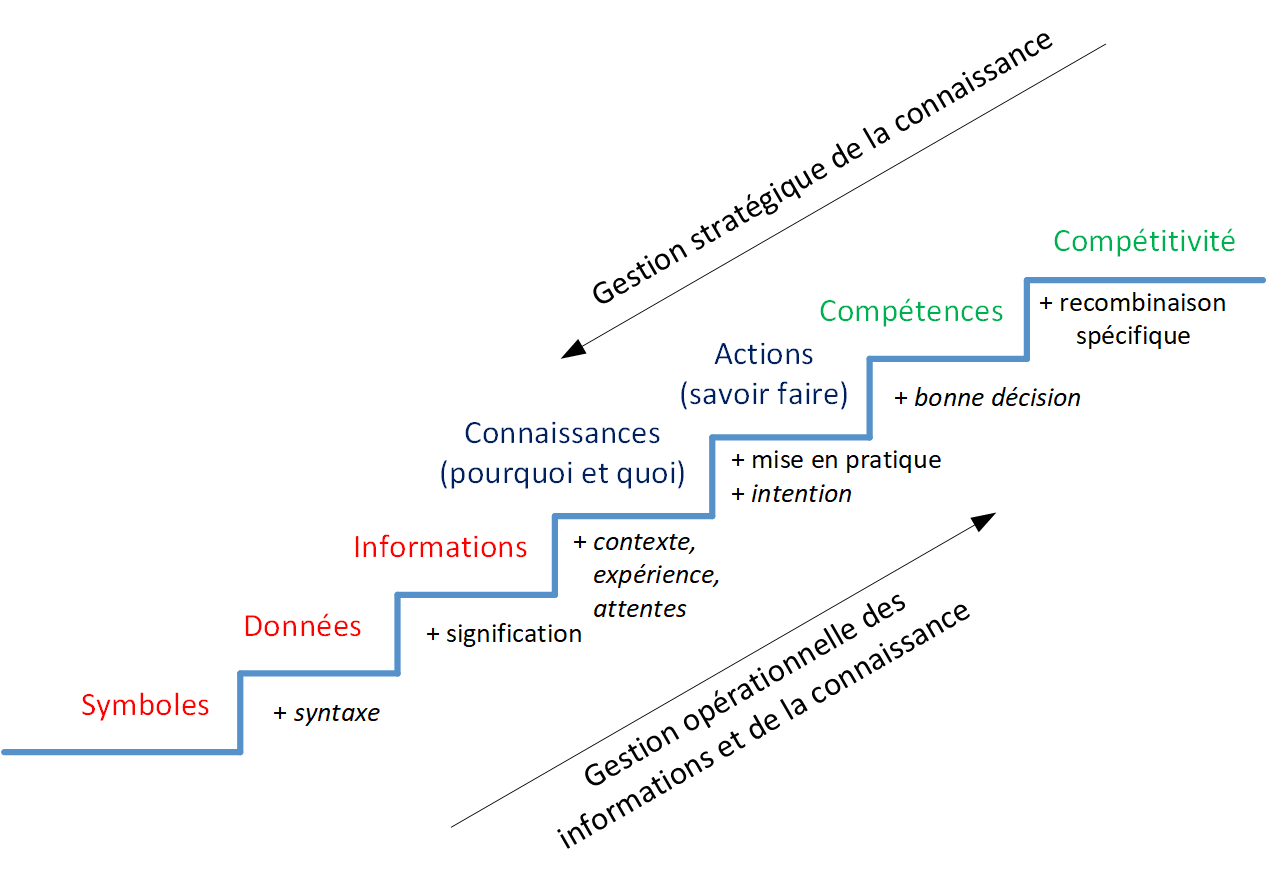
\includegraphics[scale=0.85]{2-Etat-de-l'Art/images/KM/KnowledgeLadder.png}
}
\caption{\'Echelle des connaissances traduite de~\cite{north2018knowledge}}
\label{figure:2-S1-KnowledgeLadder}
\end{figure}


\subsubsection{Connaissances tacites et explicites}
\label{subsubsection:Contexte:KIP-RevueLitterature:KM:ConnaissancesTacitesExplicites}

Les \textit{connaissances explicites} sont formalisées, structurées, systématiques, codifiées et peuvent donc aisément être manipulées, conservées, et partagées~\cite{north2018knowledge}\cite{syed2018palgrave}\cite{nonaka2007knowledge}\cite{nonaka2000seci}.
Les écrits et schémas sont les exemples typiques de connaissances explicites permettant de les transférer facilement d'un individu à l'autre.
Les aspects formel et structuré sont particulièrement visibles dans les formules mathématiques et les spécifications techniques.
Un exemple concret abordé dans~\cite{nonaka2007knowledge} concerne la conception d'une machine à pain dont le pétrissage est insatisfaisant.
Afin d'améliorer le pétrissage, un boulanger expert est observé afin de recopier sa technique et permettre à la machine de générer des pâtes d'une qualité similaire aux siennes.
Les connaissances explicites pouvant être extraites concernent les spécifications de la pâte en entrée puis en sortie, c'est-à-dire ses qualités mesurables (dureté, humidité, ...).

\bigskip

Les \textit{connaissances tacites} concernent au contraire toute l'expertise acquise par un individu au travers de ses sens et de ses facultés.
Les gestes d'un artisan, ou l'intuition issue d'expériences personnelle sont des exemples typiques de connaissances tacites~\cite{north2018knowledge}\cite{syed2018palgrave}\cite{nonaka2007knowledge}.
Ces connaissances sont particulièrement difficiles à transmettre car elles dépendent complètement de l'individu et ne peuvent pas être formalisées ou exprimées aussi facilement que les connaissances explicites.
La transmission de certaines connaissances tacites peut se faire au travers de l'apprentissage : un \textit{maître} exécute des gestes, et son \textit{apprenti} les répète jusqu'à pouvoir les maîtriser, ou au moins les répéter seul pour s'améliorer de lui-même (voire pour développer sa propre technique).
Dans l'exemple de la machine à pain et du boulanger observé~\cite{nonaka2007knowledge}, les connaissances tacites concernent la technique du pétrissage manuel.
Le boulanger peut expliquer succinctement quelques étapes, mais l'expertise précise transformant la pâte implique de répéter le geste et ressentir ses effets.
Une ingénieure a donc pratiqué la technique de pétrissage avec le boulanger pour comprendre le geste et ses effets, afin de pouvoir en déduire les parties manquantes dans la machine à pain conçue.

Appliqué à l'enseignement, on peut retrouver les connaissances qu'un enseignant souhaite transmettre à ses étudiants en s'appuyant sur des connaissances explicites (le syllabus, les notions ciblées, et le support de cours associé) et les connaissances tacites de l'enseignant (expérience personnelle en tant qu'ancien étudiant, cours déjà enseignés dans le passé, par exemple).
Les connaissances tacites constituent précisément dans ce cas une valeur ajoutée à l'enseignant : choix dans l'ordre des notions présentées, accent mis sur certaines d'entre elles selon le profil des étudiants, et explications préférées par chaque groupe d'étudiants.

\bigskip

\subsubsection{Cycle SECI}
\label{subsubsection:Contexte:KIP-RevueLitterature:KM:SECI}

Ces deux types de connaissances participent à un cycle dénommé \textit{SECI}~\cite{nonaka2007knowledge} (Socialisation, Extériorisation, Combinaison, Intériorisation) illustré par la figure~\ref{figure:2-S1-ModeleSECI}.
Ce cycle s'appuie sur les quatre façons de créer et transformer des connaissances : de tacite à tacite (socialisation), de tacite à explicite (extériorisation), d'explicite à explicite (combinaison), d'explicite à tacite (intériorisation).
Chacune de ces façons correspond à des situations particulières qui se répètent :

\bigskip

\begin{itemize}
\item Socialisation (de tacite à tacite) : Deux individus partagent des connaissances tacites par la socialisation.
Il s'agit précisément de la relation où un apprenti observe, imite, et pratique ce que le maître fait, c'est-à-dire un transfert d'expérience d'une personne à l'autre.
La socialisation repose sur l'accumulation et le transfert de connaissances tacites d'un individu à l'autre.\\

\item Extériorisation (de tacite à explicite) : L'extériorisation de connaissances tacites permet de les expliciter, c'est-à-dire les formaliser et en tirer une expérience utile à l'avenir.
Modéliser un processus est une forme d'extériorisation, tout comme décrire le déroulement d'un projet pour pouvoir apprendre des points positifs et éviter certaines erreurs.
L'extériorisation repose sur l'articulation de connaissances tacites des membres d'un groupe pour pouvoir les traduire en concepts explicites.\\

\item Combinaison (d'explicite à explicite) : Plusieurs sources de connaissances explicites, telles que des documents ou des informations, peuvent être combinées pour générer de nouvelles connaissances explicites.
Lire plusieurs rapports ou articles pour en déduire une décision stratégique ou une nouvelle piste de recherche et présenter ces résultats aux collaborateurs sont des exemples.
La combinaison repose sur la recherche et l'intégration de connaissances explicites existantes, pour pouvoir en générer de nouvelles et les diffuser aux groupes d'une organisation.\\

\item Intériorisation (d'explicite à tacite) : Une fois de nouvelles connaissances explicites reçues, un individu les intériorise en les utilisant dans ses activités.
Un ingénieur en lisant une documentation formalisée découvrira des nouveautés qu'il pourra mettre en application par la suite et se les approprier, créant des connaissances tacites.
L'intériorisation concerne un individu qui apprend de nouvelles connaissances explicites au sein d'un groupe ou d'une organisation et se les approprie par la pratique, créant ainsi des connaissances tacites.
\end{itemize}


\begin{figure}[ht]
\centering
\centerline{  % FORCE FIGURE OUTSIDE THE MARGIN !!! BUT STILL CENTERING !!!
% scale = 0.7
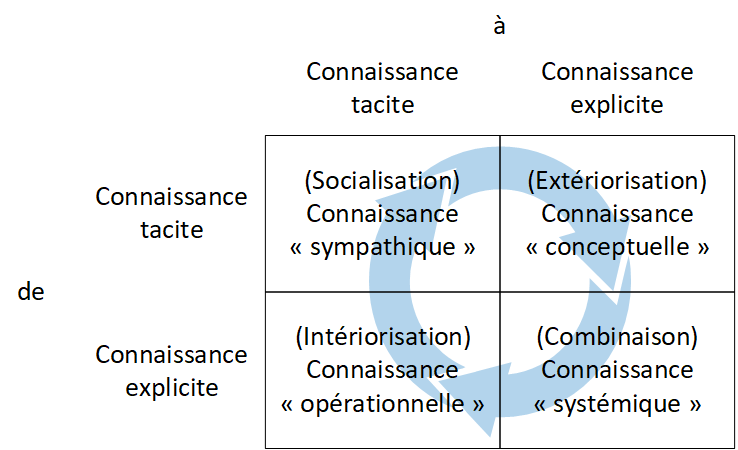
\includegraphics[scale=1]{2-Etat-de-l'Art/images/KM/ModeleSECI.png}
}
\caption{Modèle SECI de~\cite{nonaka2007knowledge} (traduction française de~\cite{tebourbi2000apprentissage})}
\label{figure:2-S1-ModeleSECI}
\end{figure}

\bigskip

Dans l'enseignement supérieur et la recherche, ce cycle se retrouve à différentes échelles.
Lors d'une conférence, des chercheurs vont présenter leurs contributions (extériorisation) et discuter les uns avec les autres (socialisation), ce qui peut engendrer la création d'une nouvelle communauté de recherche partageant des objectifs communs (combinaison) et dont chaque membre développera de nouveaux travaux selon sa propre expérience et son contexte personnel (intériorisation).

Pour un cours, les supports de cours représentent les connaissances explicites, et les échanges entre enseignant et étudiants représentent les connaissances tacites.
Un enseignant s'informera tout d'abord sur le sujet à enseigner en recherchant plusieurs sources (combinaison).
Ensuite, l'enseignant lira les sources pour s'imprégner du sujet et sélectionner les parties à présenter aux étudiants selon ses exigences (intériorisation).
Enfin, l'enseignant délivrera son cours lors de séances en travaux dirigés ou éventuellement en cours magistraux en s'appuyant sur un support de cours formel (extériorisation).
Les travaux dirigés étant particulièrement adaptés aux questions individuelles, et donc à l'apprentissage pas à pas (socialisation), cette étape est répétée en parallèle du cours magistral.
À la fin de chaque séance, l'enseignant vérifie l'avancement par rapport aux objectifs fixés (intériorisation) pour éventuellement modifier son support de cours en conséquences par rapport à ses sources (combinaison).

Inversement, du côté des étudiants, ceux-ci reçoivent un support de cours qu'ils doivent lire (intériorisation) et mettre en pratique lors des travaux dirigés (socialisation).
Les notes de cours prises (extériorisation) sont relues (combinaison) pour pouvoir se préparer aux séances suivantes.
Les notes de cours, devoirs, examens, et présentations sont des exemples de mise en forme explicite de connaissances tacites acquises.

\bigskip

L'exemple de l'enseignement montre que l'ordre des étapes n'est pas toujours rigoureusement le même, mais respecte constamment la transition entre chaque type de connaissances : les étudiants peuvent éventuellement travailler en groupe après une séance (socialisation) avant un examen (extériorisation).
Les connaissances tacites sont échangées entre camarades avant d'être explicitées dans un examen ou dans une présentation dont les membres recombineront les informations au fur et à mesure.

\bigskip

Ces activités centrées sur les connaissances, qu'elles soient tacites ou explicites, sont au c\oe{}ur de processus actuellement difficiles à gérer pour de nombreuses raisons.
Les individus et leurs connaissances tacites sont un exemple de difficulté : il est impossible de savoir à l'avance quelles connaissances tacites un individus possèdera en lui, ni les décisions qu'il prendra.
Un domaine de recherche s'intéresse en particulier aux défis posés par les connaissances dans les processus au sein des organisations, c'est-à-dire aux \textit{processus à forte intensité de connaissances}, que nous présentons dans les sous-sections suivantes.


\bigskip

%%%%%%%%%%%%%%%%%%%%%%%%%%%%%%%%%%%%%%%%%%%%
%\clearpage % Clean for pictures and tables %
%\newpage   % Clean for pictures and tables %
%%%%%%%%%%%%%%%%%%%%%%%%%%%%%%%%%%%%%%%%%%%%

\subsection{Les processus à forte intensité de connaissances}
\label{subsection:Contexte:KIP-RevueLitterature:KIP}

Observer des phénomènes se produire, c'est observer des processus s'exécuter.
Les processus tirent leurs origines linguistiques du latin \textit{processus} ou \textit{processioat} qui signifient \textit{action exécutée} ou \textit{quelque chose de fait}, et la \textit{façon dont elle a été faite}~\cite{von2014complete}.
Depuis Adam Smith et Frederick Taylor, le point de vue général adopté sur les processus métier est centré sur les activités, en particulier sur des tâches et leur ordonnancement~\cite{boissier2019challenges}.
Au sein des organisations actuelles, de nombreux processus métier sont modélisés et pris en charge par la \textit{gestion de processus métier}, ou \textit{business process management}~\cite{weske2007business} (BPM) en anglais.
Certains processus centrés sur les connaissances sont cependant encore difficiles à gérer au sein des systèmes d'informations~\cite{boissier2019challenges}, il s'agit des \textit{processus à forte intensité de connaissances}, ou \textit{knowledge intensive processes} (KIP) en anglais.
Des synonymes peuvent être retrouvés dans la littérature tels que \textit{knowledge intensive business processes}~\cite{icsik2013practices}\cite{manfreda2015knowledge} ou \textit{artful processes}~\cite{hill2006beyond}, mais certains autre termes comme \textit{case}~\cite{davenport1994case}\cite{van2005case} ont une signification un peu plus particulière que nous présentons par la suite.

\bigskip

Comme présenté dans la sous-section précédente, les connaissances tacites et explicites impliquent certaines spécificités lors de leur intégration dans les systèmes d'informations.
Les connaissances explicites sont par définition formalisées et visent à être transmises, celles-ci sont donc plus facilement intégrées aux méthodes classiques de gestion des processus.
En effet, les activités de modélisation de processus, visant à formaliser un processus en le représentant sous forme de schéma, sont déjà intégrées dans le cycle de vie du BPM et sont un exemple d'extériorisation.
Un autre exemple illustrant cette fois la combinaison concerne la rédaction des rapports annuels : les informations agrégées sont directement issues du système d'informations, parfois même de façon automatique.
À l'inverse, les connaissances tacites étant par définition informelles et uniques à chaque individu, celles-ci sont beaucoup moins aisées à gérer.
La socialisation peut éventuellement être facilitée par l'organisation d'évènements ou d'ateliers, mais l'intériorisation est au contraire une étape totalement individuelle et ne peut donc pas simplement être provoquée par une volonté extérieure.

L'étude des processus à forte intensité de connaissances s'intéresse particulièrement, mais pas exclusivement, aux connaissances tacites afin de mieux les prendre en charge et exploiter leur potentiel.
L'importance des connaissances dans ces processus leur confère plusieurs caractéristiques et exigences telles que la flexibilité dans l'ordre des activités, des évènements inattendus impliquant des tâches imprévisibles (donc absentes des modèles de processus conçus à priori), de la créativité, et bien d'autres.

\bigskip

\subsubsection{Caractéristiques des KIP}
\label{subsubsection:Contexte:KIP-RevueLitterature:KIP:CaracteristiquesKIP}

Plusieurs études ont cherché à comprendre plus en profondeur les KIP et leurs caractéristiques afin de pouvoir, si possible, les intégrer aux outils et méthodes BPM déjà en place.
Les travaux présentés dans~\cite{icsik2013practices} ont cherché dans la littérature les différences entre les KIP et les processus métier plus traditionnels.
La plupart des caractéristiques n'opposent pas directement les deux types de processus, mais les KIP en accentuent certaines.
Typiquement, \og \textit{les degrés exigés de complexité, répétabilité, et créativité ne sont pas les mêmes, mais ils ne sont pas moins éligibles à l'automatisation ou l'organisation structurée} \fg~\cite{icsik2013practices} (\og \textit{different levels of complexity, repeatability and creativity required for these processes, but are not necessarily less eligible for automation or structured} \fg~\cite{icsik2013practices}).
Cependant, l'article conclut tout de même que les KIP sont \og \textit{plus complexes, moins répétables, et exigent beaucoup de créativité} \fg~\cite{icsik2013practices}.

\bigskip

Les travaux dans~\cite{di2015knowledge} insistent tout d'abord sur les liens entre le BPM et le domaine du KM qu'il faut développer.
En effet, la connaissance est un élément clé jusque là peu exploité dans le BPM, alors qu'elle contient d'après~\cite{davenport2005thinking} \og \textit{l'expérience, le contexte, l'interprétation et la réflexion, et implique plus de coopération humaine que d'informations} \fg~\cite{di2015knowledge} (\og \textit{experience, context, interpretation and reflection and involves more human participation than information} \fg~\cite{di2015knowledge}).
Cette vision met l'accent sur les connaissances tacites, étant donné que les connaissances explicites s'appuient sur des informations et des données déjà connues des systèmes d'informations, et donc des méthodes BPM mises en place.
Plusieurs autres définitions sont également étudiées, mais une en particulier~\cite{vaculin2011declarative} insiste sur le rôle des \textit{travailleurs du savoir} (\textit{knowledge workers} en anglais) qui effectuent des tâches impliquant des prises de décisions à forte intensité de connaissances, c'est-à-dire en rassemblant de nombreuses informations pour en générer de nouvelles, voire pour produire des artefacts (par exemple des plans, des recommandations, ou encore des exigences liés aux décisions prises).
Une définition des \textit{artful processes} proposée dans~\cite{hill2006beyond} insiste également sur l'importance des individus exécutant le processus et surtout leurs connaissances tacites (\og \textit{compétences, expérience, jugement} \fg~\cite{hill2006beyond}) : le processus, voire les tâches, sont définissables d'un point de vue haut niveau, mais il est impossible de fixer à l'avance les détails.
\cite{di2015knowledge} souligne également le fait qu'un \textit{artful process} est en fait défini par les personnes (et leurs connaissances) qui l'exécutent : il n'est pas possible de définir un processus à proprement parler, mais il faut plutôt parler de l'instance en elle-même.

\bigskip

Toujours dans~\cite{di2015knowledge}, huit caractéristiques des KIPs ont été retenues et sont présentées afin d'en déduire vingt cinq exigences.
Les KIPs y sont considérés comme :
\begin{itemize}
\item Dirigés par les connaissances (\og \textit{knowledge-driven} \fg) : les données et connaissances disponibles servent à prendre les décisions et donc à diriger le processus.
\item Orientés collaboratif (\og \textit{collaboration-oriented} \fg) : le contexte d'exécution du processus est collaboratif et multi-utilisateurs, et les connaissances et artefacts générés (autant par les humains que par l'instance de processus) sont partagés.
\item Imprédictibles (\og \textit{unpredictable} \fg) : chaque instance dispose de son propre contexte et d'éléments imprévisibles qui font varier les connaissances exploitées, le flot d'exécution, et l'ordre des tâches d'une instance à l'autre.
\item Émergents (\og \textit{emergent} \fg) : l'exécution du processus fait émerger au fur et à mesure des informations qui permettent de choisir les actions et décisions à prendre.
\item Orientés buts (\og \textit{goal-oriented} \fg) : des buts intermédiaires servent à avancer dans l'exécution du processus.
\item Dirigés par les évènements (\og \textit{event-driven} \fg) : les décisions prises par les travailleurs du savoir pour avancer dans l'exécution du processus dépendent des évènements rencontrés.
\item Dirigés par les contraintes et les règles (\og \textit{constraint- and rule-driven} \fg) : les actions et décisions prises par les utilisateurs sont guidées par des règles ou contraintes à respecter.
\item Non-répétables (\og \textit{non-repeatable} \fg) : les situations variant à chaque instance de processus, il est quasiment impossible de parfaitement répéter une précédente exécution.
\end{itemize}

\bigskip

Ces caractéristiques ne sont pas exhaustives, étant donné que le domaine est toujours actif et que les tâches non-liées à un système ou environnement d'exécution BPM n'ont pas été complètement dénombrées, mais elles sont particulièrement pertinentes.
Une réunion, par exemple, implique par définition de la collaboration entre toutes et tous les participants, chaque point de l'ordre du jour doit être abordé (buts intermédiaires), elle est dirigée par les connaissances partagées au fur et à mesure des discussions et des points de vues de chacun, certains sujets seront peut être plus développés que d'autres (émergence et imprédictibilité), voire, la réunion peut être interrompue par un évènement inattendu.
Dans tous les cas, il sera impossible de répéter scrupuleusement la réunion dans sa séquence et son contenu.

Il faut tout de même retenir qu'un KIP ne répond pas nécessairement à l'ensemble de ces caractéristiques, mais au moins à certaines d'entre elles.
Le développement d'un logiciel peut tout à fait se réaliser seul (et sans utiliser de forum d'entre-aide) : il suffit d'avoir des connaissances en développement logiciel, et de respecter les limitations imposées par la machine et système d'exploitation ciblés.
Cependant, ce logiciel sera peu réutilisable en l'absence de documentation explicitant le contexte précis d'utilisation.
De plus, l'absence de prise en compte des retours utilisateurs (d'ailleurs souvent issus de \textit{l'expérience utilisateur}) limitera les évolutions.
Les différentes méthodes agiles de développement d'applications~\cite{fowler2001agile} visent justement à essayer d'intégrer au mieux toutes ces caractéristiques : fixer des buts intermédiaires régulièrement, prévoir de la collaboration entre développeurs et utilisateurs, s'adapter au changement et limiter l'impact des évènements imprévus, ... tout en essayant de produire les applications les plus réutilisables possibles mais en s'adaptant au contexte de chaque cas.


\bigskip


\subsubsection{Difficultés pour gérer les KIP}
\label{subsubsection:Contexte:KIP-RevueLitterature:KIP:DifficulteGestionKIP}

Les participants et leurs connaissances sont donc au c\oe{}ur de ces processus dont les caractéristiques précédemment relevées sont difficilement intégrables telles quelles dans l'environnement BPM classique~\cite{riss2005challenges}\cite{moura2013collaboration}.
Nous avons identifié six défis concernant les KIPs et les avons décrits dans une publication~\cite{boissier2019challenges}.

\begin{enumerate}
\item \og \textit{Comment gérer de façon efficiente et efficace les connaissances et informations manipulées (c'est-à-dire créées, utilisées, mises à jours) par les KIPs ?} \fg
L'absence de gestion des connaissances et des informations impacte négativement les KIPs.
Les travaux de~\cite{hislop2018knowledge} exposent justement les difficultés auxquelles font face dans la pratique les organisations dans la gestion des grandes quantités d'informations.
Bien que le domaine des \textit{Mégadonnées} (\textit{Big Data} en anglais) et ses 3V visent les problèmes liés aux \textit{Volume, Vélocité et Variété}, il s'agit de manipuler des \textit{données} et non pas des \textit{informations} ni des \textit{connaissances}~\cite{delort2018big}.\\

\item \og \textit{Comment supporter l'aspect collaboratif et les prises de décisions spécifiques au contexte dans les KIPs ?} \fg
Les organisations ont plutôt tendance à standardiser et contrôler les processus~\cite{riss2005challenges}, or, limiter la collaboration et la créativité limite les capacités des utilisateurs~\cite{gromoff2017business} et contrevient aux caractéristiques mêmes des KIPs.
Bien que des solutions tentent d'améliorer les communications informelles~\cite{di2011mailofmine}, l'aspect collaboratif entre les participants aux KIPs reste un défi à relever~\cite{moura2013collaboration}.\\

\item \og \textit{Comment intégrer les informations de contexte lors de la conception d'un KIP ?} \fg
Le contexte d'exécution d'un KIP sous-entend la situation ou l'environnement d'exécution (l'état de l'organisation, des équipes impliquées, ou de la société en général) ainsi que les connaissances tacites des participants au KIP.
Prévoir lors de la conception d'un processus dans quelle situation sera l'organisation et quelles seront les connaissances tacites des utilisateurs est quasiment impossible : chaque instance de KIP étant unique, des activités ou évènements inattendus peuvent se produire et apporter de nouvelles expériences aux utilisateurs qui ne répèteront pas nécessairement le même cheminement y compris si un cas similaire se reproduit.
Le paradigme déclaratif~\cite{tran2015embracing} permet à minima de proposer des règles et un cadre à respecter, mais aussi dans lequel évoluer.
Le contexte n'est donc pas complètement prévisible ni intégré, mais certaines conditions d'exécutions peuvent indiquer quelles activités faire ou préférer.\\

\item \og \textit{Comment supporter la conformité dans les KIPs ?} \fg
Par définition, le paradigme impératif du BPM simplifie la mise en place de règles de conformité.
Le domaine de la \textit{gestion de règles métier}~\cite{ross2003manifesto}, ou \textit{Business Rules Management} (BRM) en anglais, apporte une réponse particulièrement adaptée en séparant les règles des processus~\cite{zur2007business}.
Comme indiqué dans le défi précédent : le paradigme déclaratif offre des pistes pour cadrer les KIPs, mais assurer une conformité stricte de façon automatisée est encore difficile.
Le déroulement des activités dépendant surtout des décisions prises par les participants~\cite{kushnareva2015modelingStatecharts}, ces derniers ont donc majoritairement un contrôle sur le processus et donc la responsabilité concernant le respect de la réglementation.
Une autre contrainte réside aussi dans le fait que la règlementation est exprimée dans le langage naturel, voire avec des spécificités du droit, et qu'il est parfois long et difficile de les transformer en règles métier accessibles aux utilisateurs des KIPs~\cite{zur2007business}.
Quelques solutions sont néanmoins étudiées pour simplifier cette transformation~\cite{zasada2018box}.\\

\item \og \textit{Comment supporter la flexibilité dans les KIPs ?} \fg
L'imprédictibilité et la créativité, mais aussi l'émergence et les évènements se produisant au fil du temps, impliquent que les utilisateurs de KIPs ont besoin d'une grande liberté d'action.
Comme nous l'avons vu, il s'agit cependant aussi de restreindre cette liberté selon les réglementations du domaine, voire, les contraintes liées au contexte particulier du cas étudié.
La flexibilité nécessaire pour entretenir une certaine liberté d'action, tout en respectant les contraintes, est grandement étudiée dans la littérature~\cite{riss2005challenges}\cite{herrmann2011adaptive}\cite{huber2015adaptive}\cite{tran2015embracing}\cite{de2016modeling}\cite{gromoff2017business}\cite{zensen2018comparison}, car il s'agit d'un problème encore ouvert.\\

\item \og \textit{Comment explorer et réutiliser des fragments de processus dans les KIPs ?} \fg
Le domaine du \textit{raisonnement à base de cas}~\cite{slade1991case}, ou \textit{Case-Based Reasoning} (CBR) en anglais, vise à ré-\og \textit{utiliser les expériences passées pour comprendre et résoudre de nouveaux problèmes} \fg~\cite{kolodner1992introduction} (\og \textit{using old experiences to understand and solve new problems} \fg~\cite{kolodner1992introduction}).
Cette idée a été étudiée dans quelques travaux~\cite{di2015knowledge}\cite{cognini2016case} en proposant aux utilisateurs des KIPs des \textit{motifs} (ou \textit{patterns} en anglais) issus d'instances précédemment exécutées.
La validation des motifs par des experts du domaine peut permettre leur réutilisation en accord avec les règles en place.
Ces motifs, selon leur nature, peuvent également embarquer une partie du contexte des exécutions précédentes sans intervention manuelle, et donc répondre à plusieurs défis précédemment énoncés.\\

\end{enumerate}

\bigskip

Comme nous venons de le voir, les KIPs font encore face à de nombreux défis partiellement interdépendants.
Plusieurs domaines de recherche connexes contribuent à affiner les réponses possibles, mais ne permettent pas en l'état d'intégrer les KIPs aux systèmes d'informations s'appuyant uniquement sur le BPM.
La littérature propose plusieurs points de vues sur les KIPs permettant de mieux se concentrer sur certains défis.



\bigskip

%%%%%%%%%%%%%%%%%%%%%%%%%%%%%%%%%%%%%%%%%%%%
%\clearpage % Clean for pictures and tables %
%\newpage   % Clean for pictures and tables %
%%%%%%%%%%%%%%%%%%%%%%%%%%%%%%%%%%%%%%%%%%%%

\subsection{Le défi de la réutilisation des fragments de processus et des connaissances}
\label{subsection:Contexte:KIP-RevueLitterature:Reutilisation}

Le raisonnement à base de cas~\cite{slade1991case}\cite{kolodner1992introduction} s'appuie énormément sur la réutilisation des cas passés afin d'en résoudre de nouveaux.
Ce point de vue des cas est issu de la \textit{gestion de cas}~\cite{davenport1994case}\cite{van2005case}\cite{swenson2013white}, ou \textit{case management} en anglais, qui s'appuie sur des pratiques où l'ensemble des informations nécessaires pour réaliser des activités sont rassemblées dans ce qui s'appelle un \textit{cas}~\cite{swenson2013white}.
L'expérience acquise lors d'une activité se répercute dans les connaissances tacites des individus impliqués, et éventuellement sous forme explicite si des traces ou des artefacts ont été générés.
Il s'agit de l'intériorisation dans le cycle SECI présenté précédemment : chaque individu a pratiqué une activité en s'appuyant sur des connaissances explicites qui sont devenues progressivement tacites.
Ces connaissances tacites sont cependant uniques à la situation dans laquelle s'est réalisée l'activité.
Réutiliser ces connaissances implique que l'individu se retrouve dans une situation similaire, c'est-à-dire que le contexte soit suffisamment proche pour qu'il puisse adapter ses actions.

La réutilisation des connaissances est étudiée dans la littérature, mais beaucoup moins que plusieurs autres étapes intervenant avant la réutilisation en elle-même~\cite{schacht2016methodology} que nous décrivons par la suite.
Du point de vue des processus à forte intensité de connaissances, les fragments de processus permettent de s'appuyer sur l'expérience des individus dans leurs activités pour extraire un sous-ensemble de tâches et activités afin de les réutiliser lors de la conception et de l'exécution.


\bigskip


\subsubsection{Le défi de la réutilisation dans le cas de la gestion des connaissances connaissances}
\label{subsubsection:Contexte:KIP-RevueLitterature:ReutilisationKIP:KM}


Les travaux présentés dans~\cite{markus2001toward} étudient la réutilisation de connaissances sous sa forme de processus avec des rôles et des dépôts de connaissances, pour en déduire quatre types de situations de réutilisation possibles.
Le processus général de gestion des connaissances se divise en quatre étapes :

\begin{enumerate}
\item Capturer ou documenter les connaissances (\og \textit{capturing or documenting knowledge} \fg) : documentation de(s) l'activité(s) par des moyens automatiques ou induits par l'activité(s) elle(s)-même(s) (archivage automatique de messages échangés, par exemple), ou par des structures prévues à la conception (champs obligatoires à remplir, par exemple).\\

\item Empaqueter les connaissances à réutiliser (\og \textit{packaging knowledge for reuse} \fg) : les documents générés sont nettoyés puis mis en forme pour pouvoir être indexés dans un dépôt.
Les informations concernant le contexte sont ajoutées, le contenu des documents est filtré et nettoyé, et des modèles de classification sont développés.\\

\item Distribuer ou disséminer les connaissances (\og \textit{distributing or disseminating knowledge} \fg) : partage des connaissances de façon passive (dépôt alimenté régulièrement par les nouvelles expériences, ou envoi régulier d'une note d'informations, par exemple) ou active (organisation de réunions détaillant un retour d'expérience particulier, par exemple), et activités de facilitation (aide à l'utilisation ou à l'identification de besoins en réutilisation de connaissances, ou mise en place de bonnes pratiques, par exemple).\\

\item Réutiliser les connaissances (\og \textit{reusing knowledge} \fg) : Cette dernière étape se décompose elle-même en quatre activités.
Tout d'abord, \textit{définir la question} (\og \textit{defining the search question} \fg) afin de mobiliser les connaissances et experts les plus aptes à y répondre.
Puis, \textit{chercher et localiser les experts ou les expertises} (\og \textit{the search for, and location of, experts or expertise} \fg), pour pouvoir ensuite \textit{sélectionner l'expert ou le conseil approprié d'un expert} (\og \textit{selection of an appropriate expert or of expert advice} \fg).
Enfin, \textit{appliquer les connaissances} (\og \textit{applying the knowledge} \fg) à la situation actuelle, c'est-à-dire en recontextualisant les connaissances récupérées du dépôt.
Cette dernière étape s'appuie sur deux notions spécialisées sur les connaissances : le \textit{rappel} (\og \textit{recall} \fg) qui permet de savoir si une information a été indexées et la retrouver, et la \textit{reconnaissance} (\og \textit{recognition} \fg) qui permet de savoir si une information répond aux besoins de l'utilisateur et s'applique aux connaissances visées.
Mais aussi sur deux notions spécialisées sur l'expertise humaine : l'\textit{identification} (\og \textit{identification} \fg) d'experts sur un domaine en particulier, et la \textit{sélection} (\og \textit{selection} \fg) de l'expert le plus approprié pour la question.
\end{enumerate}


\bigskip

Trois rôles sont également mobilisés lors de l'exécution de ce processus de réutilisation~\cite{markus2001toward}.
Ces rôles peuvent être tenus par des individus distincts, ou par le même :

\begin{itemize}
\item Producteur de connaissances (\og \textit{knowledge producer} \fg) : la personne qui documente les connaissances en enregistrant les connaissances explicites, ou en transformant les connaissances tacites en connaissances explicites (extériorisation).

\item Intermédiaire de connaissances (\og \textit{knowledge intermediary} \fg) : la personne qui adapte les connaissances pour les réutiliser grâce à l'élucidation, le nettoyage, l'indexation, et l'empaquetage.
Cette personne est également chargée de distribuer les connaissances au sein de l'organisation.

\item Consommateur de connaissances (\og \textit{knowledge consumer} \fg) : la personne qui retrouve et adapte le contenu des connaissances passées pour les appliquer à son cas.
\end{itemize}

\bigskip

De nombreux types de dépôts existent dont les caractéristiques les distinguent les uns des autres~\cite{markus2001toward}.
La plus simple des distinctions s'appuie sur la nature des objets entreposés : les \textit{documents} (texte, audio, vidéo) n'étant pas toujours stockés de la même manière que les \textit{données} (structures de données, systèmes de gestion de base de données relationnelles / SGBDR).
Les travaux dans~\cite{davenport1998successful} distinguent les \textit{connaissances externes}, concernant l'environnement extérieur à l'organisation, les \textit{connaissances internes structurées}, tels que les documents et données, et enfin les \textit{informations informelles}, comme les notes de réunions ou les mails.
Une autre distinction présentée dans~\cite{zack1999managing} concerne la nature des connaissances : les \textit{connaissances générales}, tel que l'état des connaissances scientifiques actuelles, et les \textit{connaissances spécifiques}, tels que les informations et le vocabulaire internes à une organisation.

Dans le contexte actuel où les données et informations sont accessibles quasiment n'importe où, ces dépôts peuvent être assimilés à d'autres formes que les \textit{entrepôts de données} (\og \textit{date warehouses} \fg) ou SGBD traditionnels, comme par exemple les nombreux \textit{wikis}~\cite{schacht2016methodology}.

\bigskip

Ce processus, les rôles, et les dépôts représentent un modèle général de gestion des connaissances dans lequel l'étape de réutilisation intervient relativement tard.
La réutilisation de connaissances implique évidemment de créer et stocker des connaissances, avant de les partager ou de les transférer et éventuellement de les adapter.
Quatre types de situations de réutilisation des connaissances ont été identifiés et sont présentés dans une typologie~\cite{markus2001toward} :

\begin{itemize}
\item \textit{Producteurs collaboratifs} (\og \textit{Shared Work Producers} \fg) : les individus travaillant dans des équipes proches les unes des autres produisent, stockent, partagent et retrouvent leurs propres connaissances pour les réutiliser.
Bien qu'ils n'aient que peu de difficultés à réutiliser leurs connaissances, lorsque les équipes en question stockent beaucoup trop de connaissances, il est parfois difficile et long de retrouver précisément celles recherchées.
Le problème se pose également lorsque ces connaissances ne sont pas numérisées (des brouillons, par exemple) ou qu'elles sont mal renseignées lors de leur enregistrement (contexte mal détaillé).\\

\item \textit{Praticiens collaboratifs} (\og \textit{Shared Work Practitioners} \fg) : les individus affectés à une même fonction mais éloignés géographiquement, dans l'organigramme, ou bien même dans des organisations distinctes, partagent néanmoins des connaissances qu'ils réutilisent.
Les principales difficultés concernent la sélection des connaissances les plus adaptées au problème (les consommateurs n'arrivent pas à évaluer quelles connaissances répondent au mieux à leurs besoins), la réputation des contributeurs (certains contributeurs seront préférés à d'autres), enfin le contexte des connaissances (les consommateurs de connaissances peuvent ne pas connaître ni comprendre le contexte d'origine).\\

\item \textit{Novices cherchant une expertise} (\og \textit{Expertise-Seeking Novices} \fg) : les individus étrangers à un domaine ont besoin d'experts pour les aider à réutiliser des connaissances.
De nombreuses difficultés sont rencontrées par les novices, dont la première est le jargon (la question posée ne contient pas le ou les termes spécifiques qui permettraient de comprendre le problème et retrouver immédiatement les connaissances adaptées), suivie du contexte des informations (un novice peut mélanger le contexte et les informations), et enfin les connaissances doivent être présentées de façon accessible aux non-experts (renvoyer des débutants vers un manuel technique complet ne leur permet pas d'identifier précisément la connaissance recherchée).\\

\item \textit{Explorateurs tiers de connaissances} (\og \textit{Secondary Knowledge Miners} \fg) : les individus effectuant de l'exploration de données peuvent également réutiliser des connaissances et en générer de nouvelles.
Ces utilisateurs ne connaissent pas toujours le contexte exact dans lequel les données ont été extraites ni l'objectif initial.
Il est donc conseillé de fournir une formation solide aux utilisateurs effectuant de l'exploration de données afin qu'ils maîtrisent les limites des ensembles qu'ils manipulent.
\end{itemize}

\bigskip

La plupart des réponses pour dépasser ces limites concernent la documentation : documenter pour soi-même afin de pouvoir retrouver, comprendre, et réutiliser ses propres connaissances, documenter pour les pairs du domaine afin de les orienter vers les connaissances les plus adaptées, et enfin documenter pour les novices afin de leur permettre d'adapter les connaissances à leur cas (en retirant l'excès de contexte avant de les leur fournir) et d'éviter l'excès de données pouvant entraîner de mauvaises interprétations.
Concrètement, dans les projets informatiques actuels, on peut retrouver cette documentation dans les commentaires d'un code, dans les notes des outils de gestion de versions, voire dans les wikis.

\bigskip

D'autres travaux~\cite{petter2009developing} décrivent trois méthodes de réutilisation observées dans le cas des projets informatiques d'une société de conseils :

\begin{itemize}
\item Le \textit{verbatim} (\og \textit{verbatim} \fg) : les connaissances sont directement réutilisées sans aucune adaptation (en répétant par exemple rigoureusement les mêmes étapes).
Cette méthode ne fonctionne pas toujours étant donné que les situations varient constamment et qu'il est difficile de retrouver un contexte suffisamment proche pour que les connaissances soient parfaitement réutilisables telles quelles.
Cependant, l'usage du verbatim à des fins heuristiques a fonctionné (par exemple estimer la durée d'exécution d'une tâche à partir d'exécutions passées).\\

\item La \textit{synthèse} (\og \textit{synthesis} \fg) : plusieurs sources de connaissances sont combinées afin de construire une solution adaptée au cas présent (plusieurs expériences similaires passées sont analysées ainsi qu'une liste de bonnes pratiques, afin de résoudre un nouveau problème).
Cette méthode s'appuie à la fois sur des connaissances explicites et les connaissances tacites de l'individu construisant sa solution.
L'intérêt majeur repose sur le fait que des réponses proches existent déjà, et que l'on ne construit pas une réponse à partir de rien.\\

\item La \textit{création} (\og \textit{creation} \fg) : une nouvelle solution est construite à partir de rien en effectuant des sessions de réflexion ou des réunions, c'est-à-dire en s'appuyant sur la sagesse collective.
Cette méthode est surtout utilisée dans les situations difficiles, et lorsque les autres méthodes ne fonctionnent pas.
Les réunions permettent d'exposer les problèmes et exigences à respecter pour en déduire de nouvelles solutions et leurs conséquences grâce à l'expérience de chaque individu (la simple combinaison de solutions passées n'est pas suffisante, et il est nécessaire de reprendre le problème depuis le début).
\end{itemize}

\bigskip

L'étude menée dans~\cite{ajmal2008knowledge} a montré que les solutions déployées servaient principalement à accumuler les connaissances et n'étaient jusque là que peu utilisées en pratique.
De plus, selon~\cite{schacht2016methodology}, les chercheurs et les praticiens s'intéressent plutôt à la collecte, au stockage, et au transfert de connaissances plutôt qu'à la réutilisation.
Plus précisément, l'analyse faite par~\cite{schacht2016methodology} explique que les études réalisées avec une méthodologie orientée \textit{behavior} visent à expliquer et comprendre les phénomènes, mais elles ne donnent aucune recommandation pour les praticiens.
À l'inverse, les solutions construites avec une méthodologie \textit{science du design} sont trop orientées vers les fonctionnalités, et elles ne vérifient donc pas les conséquences sur l'organisation ou les comportements des individus.

\bigskip

Du point de vue de la gestion des connaissances, la réutilisation des connaissances est donc un problème encore ouvert.
Peu de travaux de recherche s'y sont spécifiquement intéressés, et les solutions techniques proposent des fonctionnalités plutôt liées aux activités avant la réutilisation (c'est-à-dire l'acquisition, le stockage, et le transfert).


\bigskip


\subsubsection{Le défi de la réutilisation de fragments de processus dans le cas des processus à forte intensité de connaissances}
\label{subsubsection:Contexte:KIP-RevueLitterature:Reutilisation:KIP}

Dans le domaine des processus à forte intensité de connaissances, la réutilisation de fragments est également un des défis actuellement étudiés~\cite{boissier2019challenges}.
Les travaux de~\cite{eberle2009process}\cite{eberle2010process} donnent une définition des \textit{fragments de processus} en indiquant qu'il s'agit des activités, et des connaissances qui y sont attachées, auxquelles chaque participant au processus est assigné selon son propre contexte local.
La notion \textit{locale} est importante dans le sens où chaque fragment est lié à la fois à une partie d'un processus (un sous-ensemble d'activités), à un individu exécutant les activités impliquées, et aux connaissances mobilisées à l'exécution de ces activités.
Lors de l'inscription d'un étudiant à l'université par exemple, l'étudiant dispose de son propre fragment sur l'expérience utilisateur, les personnels administratifs des inscriptions vérifient et répondent, et enfin, les personnels administratifs des unités des formation et de recherche attribuent un groupe à chaque étudiant selon les filières.
La figure~\ref{figure:2-S1-KIP-Exemple-Fragments} expose les trois fragments de ce processus d'inscription.
Chaque fragment mobilise donc des connaissances spécifiques : générer les pièces de son propre dossier, vérifier la validité des pièces et cas particuliers puis envoyer les documents réponses, construire les groupes d'étudiants selon les exigences de la formation et des salles disponibles.
L'objectif des travaux présentés dans~\cite{eberle2010process} visent à proposer à un expert de réutiliser des fragments de processus structurés lors de la conception des processus, mais également lors de leur exécution.


%\begin{figure*} % Figure flottante
\begin{figure}[ht]
\centering
\centerline{
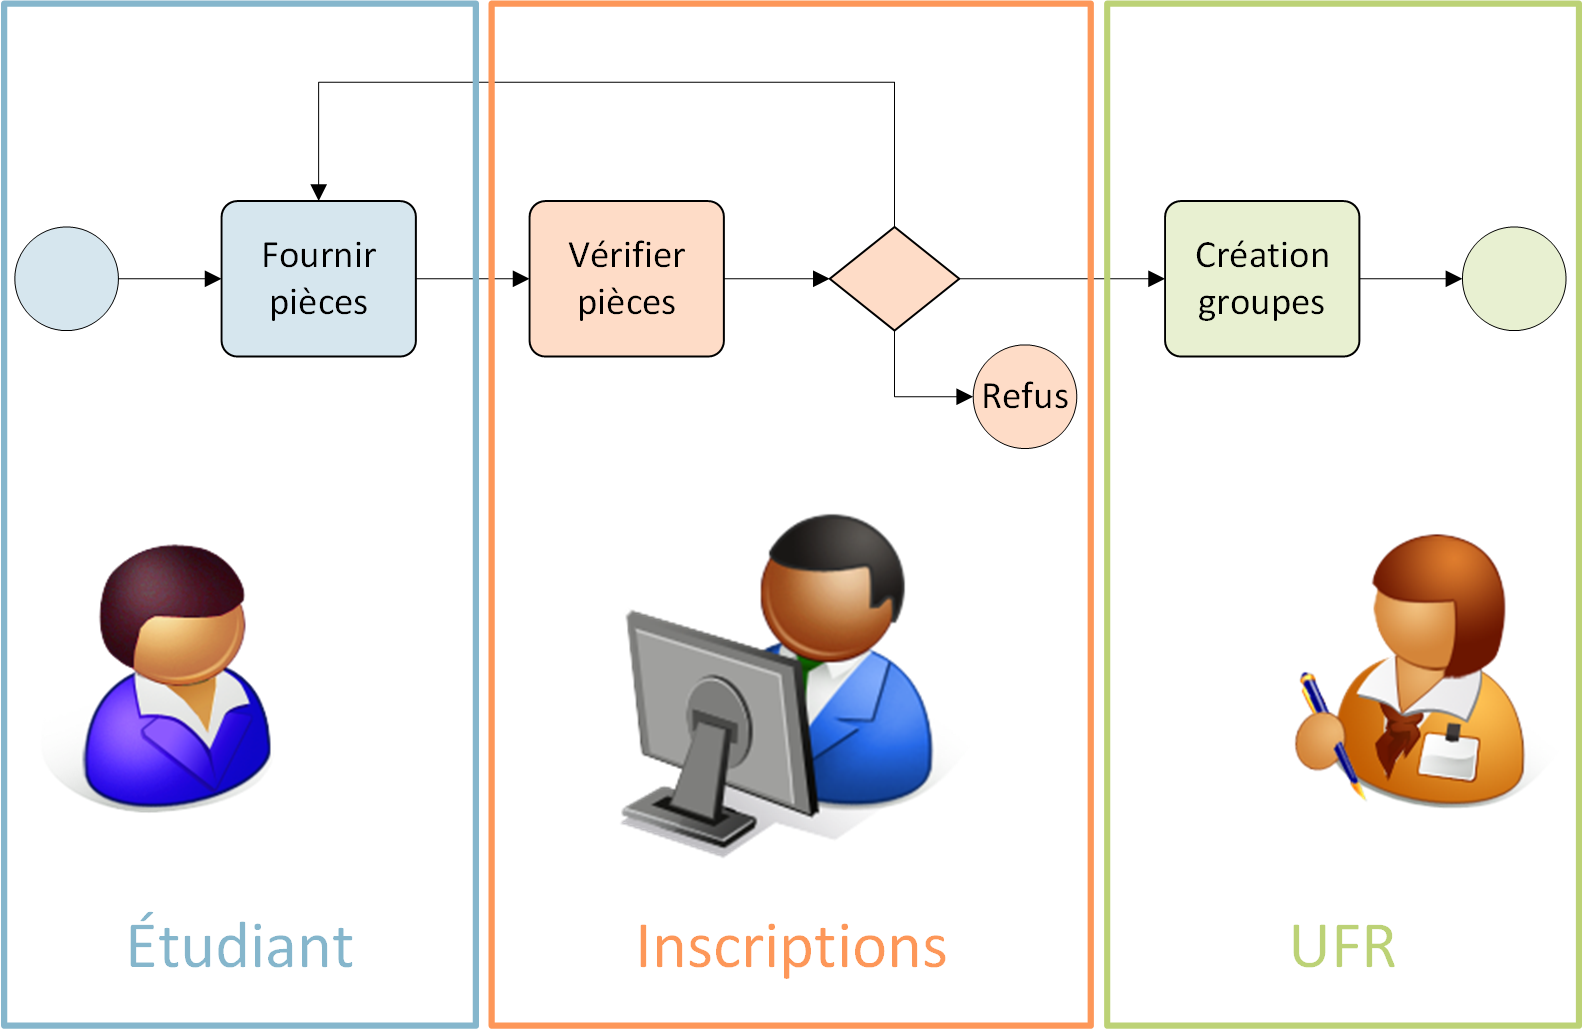
\includegraphics[scale=0.65]{2-Etat-de-l'Art/images/KIP/Fragments/FragmentsProcessus.png}
}
\caption{Exemple d'un processus d'inscription d'étudiant et de ses trois fragments}
\label{figure:2-S1-KIP-Exemple-Fragments}
\end{figure}
%\end{figure*} % Figure flottante
% To use it : fig~\ref{label}

\bigskip

Une amélioration de l'usage de ces fragments de processus a été proposée dans les travaux présentés dans~\cite{cognini2016case} en s'inspirant des techniques de CBR~\cite{slade1991case}\cite{kolodner1992introduction} afin de gérer des cas, et non plus des processus structurés.
Le CBR s'appuie sur un schéma en plusieurs étapes rappelant énormément celui appliqué en gestion des connaissances :
\begin{enumerate}
\item une personne décrit tout d'abord au système le problème auquel elle est confrontée,
\item le système recherche les cas similaires dans sa base de cas,
\item le système sélectionne le cas le plus proche afin de le réutiliser,
\item le système adapte le cas retenu au contexte actuel,
\item si la personne valide le cas adapté, celui-ci est retenu et est conservé à son tour pour un possible ré-usage futur.
\end{enumerate}

\bigskip

Les systèmes de gestion des cas s'étant développés dans un environnement statique et contrôlé, ils ne sont pas adaptés aux situations exigeant de la flexibilité~\cite{motahari2013adaptive}.
Ainsi, l'\textit{Adaptive Case Management} (ACM)~\cite{swenson2010mastering} s'est développé pour pouvoir s'affranchir des contraintes et permettre aux participants d'adapter le système aux cas rencontrés et aux évènements émergents.
La figure~\ref{figure:2-S1-KIP-Exemple-ACM} illustre la différence entre le point de vue classique impératif où un processus est modélisé de façon détaillée, et les traces d'exécutions contiennent la progression des instances, tandis que le point de vue cas s'intéresse aux intervenants qui les traitent en consultant, ajoutant, modifiant, ou supprimant des données au fur et à mesure.

\begin{figure}[ht]
\centering
\centerline{
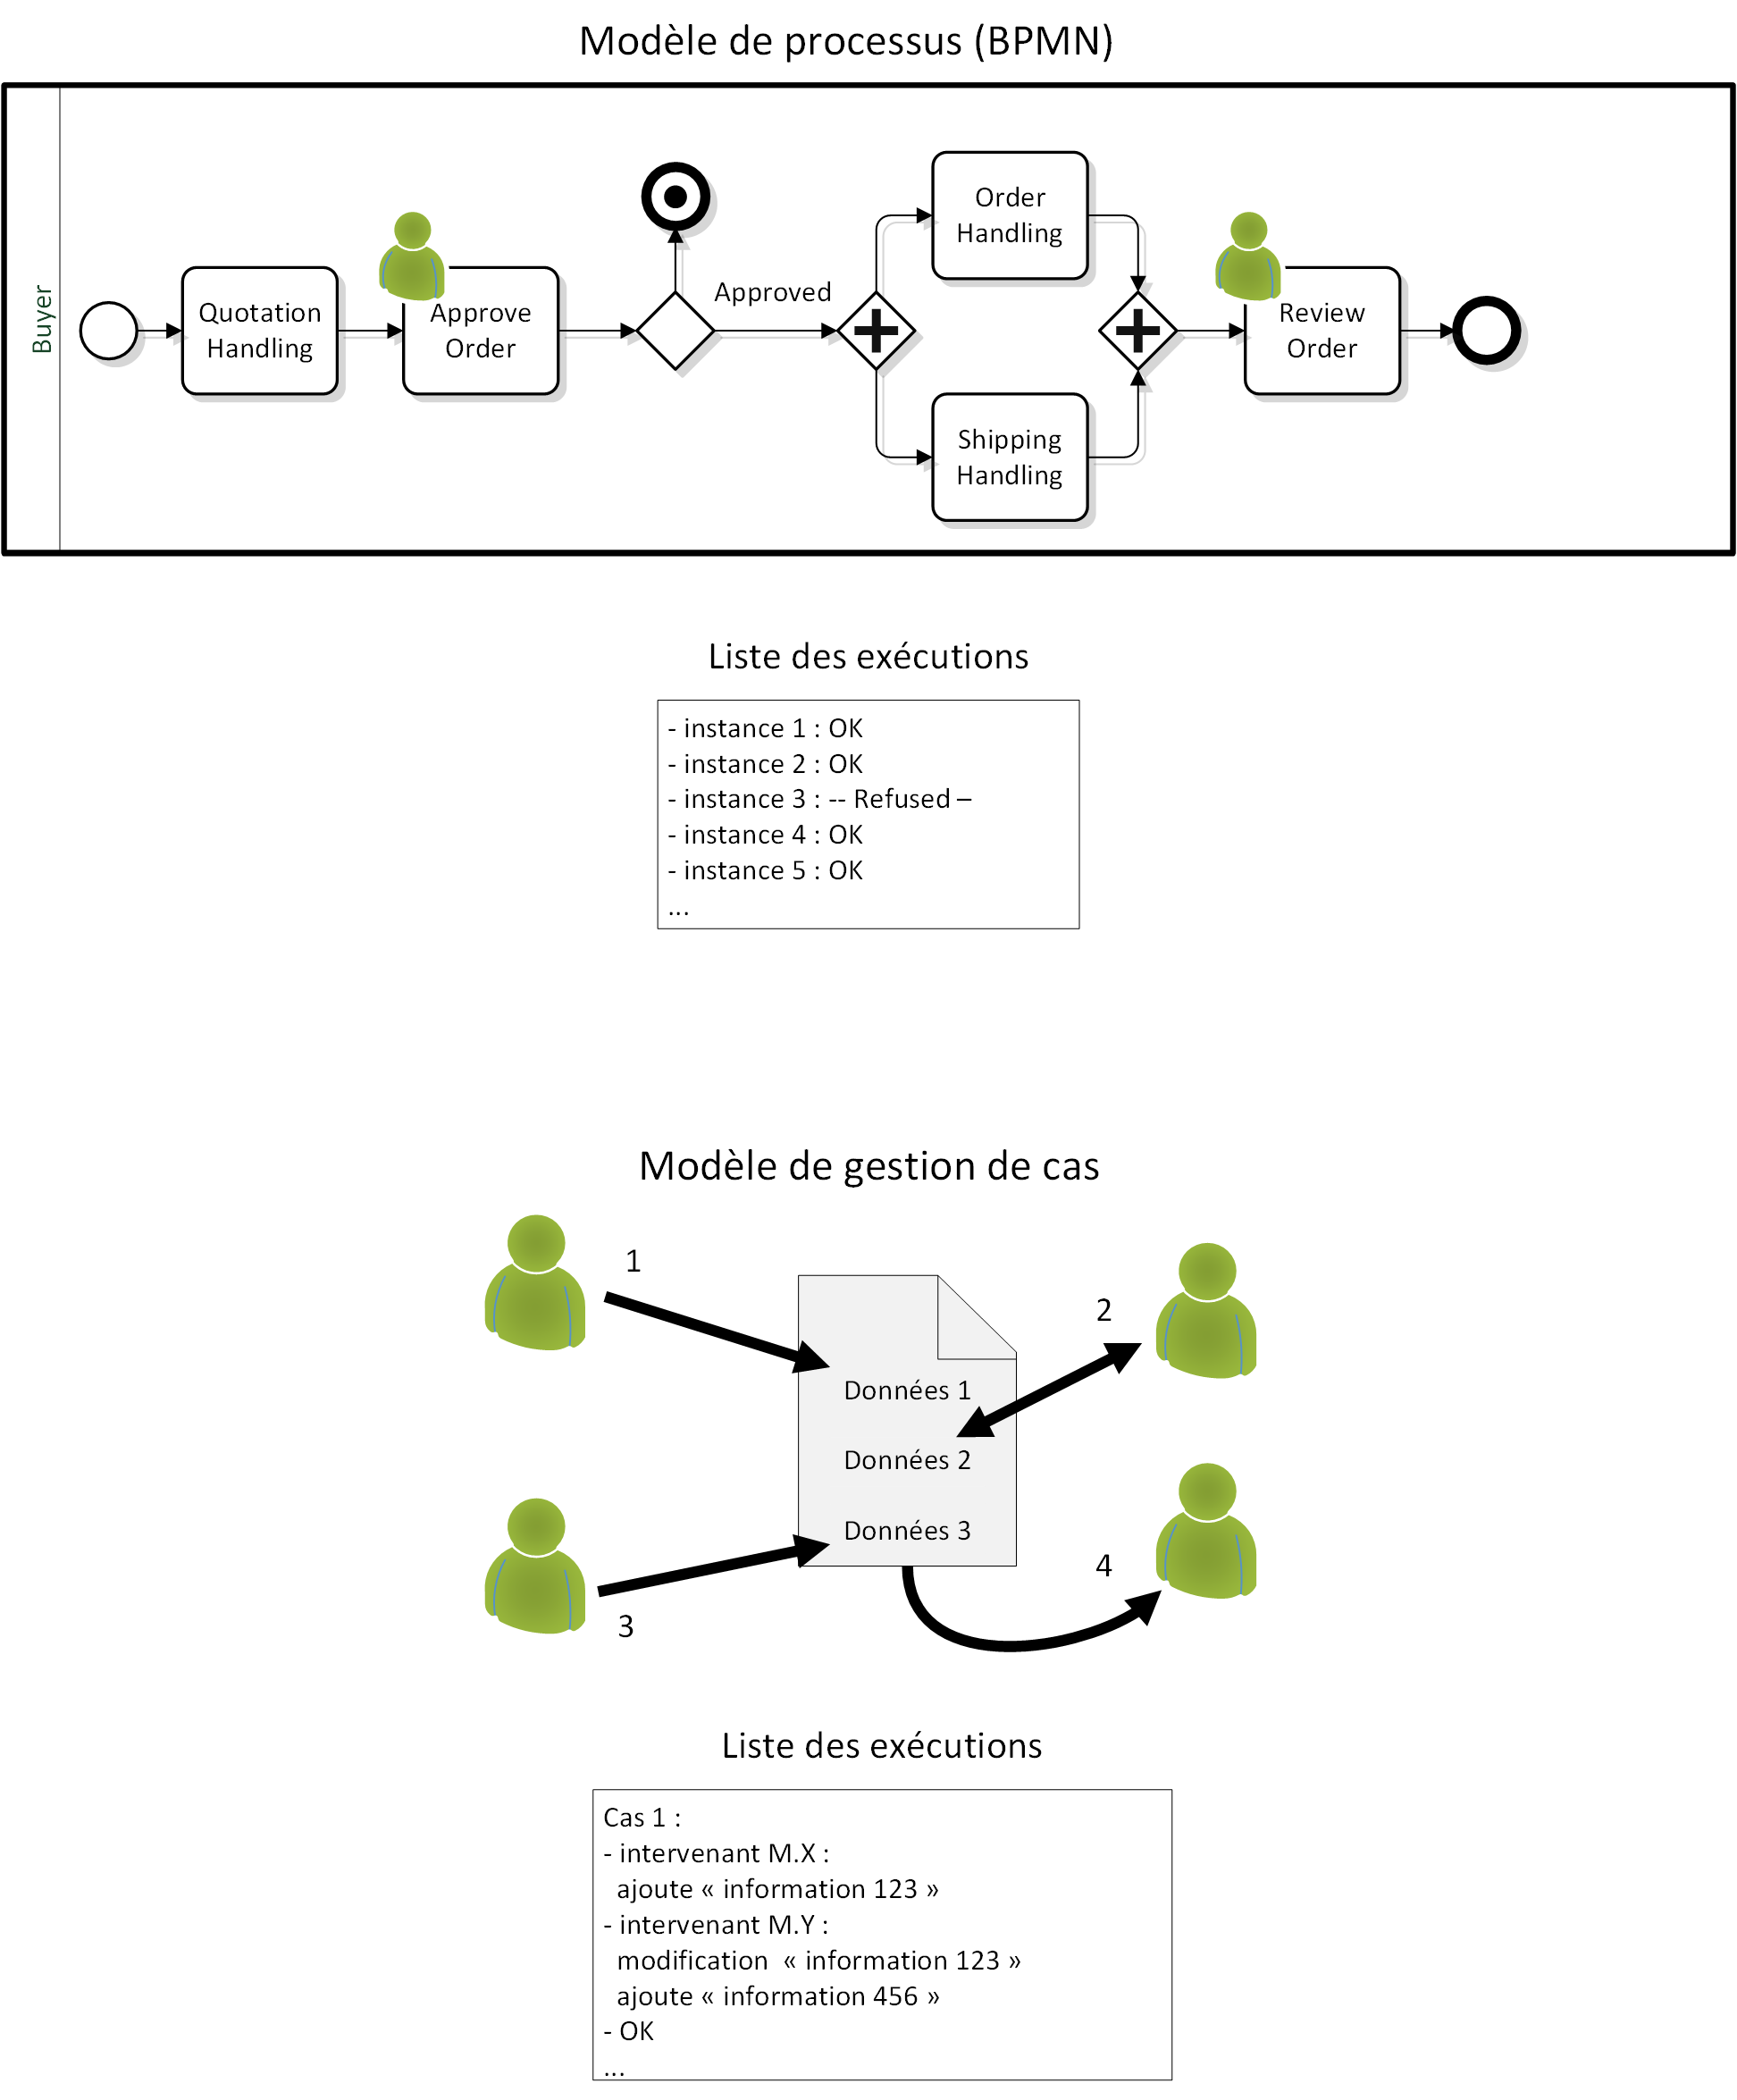
\includegraphics[scale=0.65]{2-Etat-de-l'Art/images/KIP/ACM/Exemple_Cas_vs_BPMN_hauteur.png}
}
\caption{Comparaison des point de vues impératif (BPMN) et gestion de cas}
\label{figure:2-S1-KIP-Exemple-ACM}
\end{figure}


\bigskip

L'ACM est un candidat naturel au traitement des processus à forte intensité de connaissances, de par sa nature à être dirigé par les données et les connaissances, mais également car il s'intéresse aux instances de ces processus, c'est-à-dire les cas.
La différence majeure entre l'ACM et la gestion des connaissances provient du point de vue choisi : il s'agit non pas d'étudier comment les connaissances ou données sont traitées pour en proposer d'autres et les réutiliser, mais bien de traiter des cas et les résoudre grâce à d'anciens cas avec leurs connaissances et données.
L'élément central est le cas, qui sera résolu en s'appuyant sur les connaissances des experts et les données qu'ils produisent et manipulent.
La réutilisation des cas passés, ainsi que des connaissances et données qu'ils embarquent, permet donc de simplifier la gestion des processus à forte intensité de connaissances.





%%%%%%%%%%%%%%%%%%%%%%%%%%%%%%%%%%%%%%%%%%%%%%%%%%%%%%%%%%%%%%%%%%%%%%%%%%%%%%%%%%%%%%%%%%
%%%%%%%%%%%%%%%%%%%%%%%%%%%%%%%%%%%%%%%%%%%%%%%%%%%%%%%%%%%%%%%%%%%%%%%%%%%%%%%%%%%%%%%%%%
%%%%%%%%%%%%%%%%%%%%%%%%%%%%%%%%%%%%%%%%%%%%%%%%%%%%%%%%%%%%%%%%%%%%%%%%%%%%%%%%%%%%%%%%%%
%%%%%%%%%%%%%%%%%%%%%%%%%%%%%%%%%%%%%%%%%%%%%%%%%%%%%%%%%%%%%%%%%%%%%%%%%%%%%%%%%%%%%%%%%%
%%%%%%%%%%%%%%%%%%%%%%%%%%%%%%%%%%%%%%%%%%%%%%%%%%%%%%%%%%%%%%%%%%%%%%%%%%%%%%%%%%%%%%%%%%
%%%%%%%%%%%%%%%%%%%%%%%%%%%%%%%%%%%%%%%%%%%%%%%%%%%%%%%%%%%%%%%%%%%%%%%%%%%%%%%%%%%%%%%%%%

%%%%%%%%%%%%%%%%%%%%%%%%%%%%%%%%%%%%%%%%%%%%
\clearpage % Clean for pictures and tables %
\newpage   % Clean for pictures and tables %
%%%%%%%%%%%%%%%%%%%%%%%%%%%%%%%%%%%%%%%%%%%%

%%%%%%%%%%%%%%%%%%%%%%%%%%%%%%%%%%%%%%%%%%%%%%%%%%%%%%%%%%%%%%%%%%%%%%%%%%%%%%%%%%%%%%%%%%
%%%%%%%%%%%%%%%%%%%%%%%%%%%%%%%%%%%%%%%%%%%%%%%%%%%%%%%%%%%%%%%%%%%%%%%%%%%%%%%%%%%%%%%%%%
%%%%%%%%%%%%%%%%%%%%%%%%%%%%%%%%%%%%%%%%%%%%%%%%%%%%%%%%%%%%%%%%%%%%%%%%%%%%%%%%%%%%%%%%%%
%%%%%%%%%%%%%%%%%%%%%%%%%%%%%%%%%%%%%%%%%%%%%%%%%%%%%%%%%%%%%%%%%%%%%%%%%%%%%%%%%%%%%%%%%%
%%%%%%%%%%%%%%%%%%%%%%%%%%%%%%%%%%%%%%%%%%%%%%%%%%%%%%%%%%%%%%%%%%%%%%%%%%%%%%%%%%%%%%%%%%
%%%%%%%%%%%%%%%%%%%%%%%%%%%%%%%%%%%%%%%%%%%%%%%%%%%%%%%%%%%%%%%%%%%%%%%%%%%%%%%%%%%%%%%%%%


\section{Techniques d'analyse de données}
\label{section:Contexte:TechniquesAnalyseDonnees}

Lors de la construction d'un cours, un enseignant utilise des connaissances implicites, grâce à son expérience personnelle, pour sélectionner les notions enseignées et les enchaîner de façon logique et la plus intuitive possible pour les étudiants.
L'enchaînement de notions étant lui-même un ensemble de connaissances implicites, on constate que la production de connaissances à première vue explicites repose en réalité sur de nombreuses connaissances implicites (à la fois utilisées lors du processus de création, et dans la production finale).
La réutilisation implique donc des traitements spécifiques pour analyser les connaissances embarquées dans les processus à forte intensité de connaissances et les documents qui y sont attachés.
Dans cette section, nous présentons plusieurs techniques permettant de traiter ces connaissances et les données sur lesquelles elles s'appuient.


\bigskip

Les documents étant composés de textes en langage naturel, il est tout d'abord nécessaire de les analyser avec des techniques adaptées issues du domaine du \textit{traitement automatique du langage}.
Une fois les textes analysés, et leur contenu extraits, on peut y rechercher des connaissances implicites grâce à l'\textit{analyse de concepts formels} et deux \textit{métriques dédiées}.
Une première métrique (l'\textit{impact mutuel}) permet d'estimer la pertinence des documents insérés en entrées, tandis qu'une autre (la \textit{similarité conceptuelle}) est utilisée pour construire des \textit{clusters} de termes.
Ces clusters représentent les séances sous forme d'ensemble de notions les plus proches selon les connaissances implicites exploitées par l'analyse de concepts formels.


\bigskip


\subsection{Traitement Automatique du Langage}
\label{subsection:Contexte:TechniquesUtilisees:TAL}

Comme nous l'avons vu, l'une des spécificités des KIP est de manipuler (ou faire intervenir de façon plus subtile) des connaissances, tout comme ACM se concentre sur les données des cas.
Ces connaissances et données se transmettent par des signes et des langages étudiés par plusieurs domaines comme la sémiologie ou sémiotique~\cite{goosse2016bon}.
L'approche présentée dans cette thèse visant en particulier l'enseignement supérieur, donc des activités proprement humaines où les textes sont prédominants, nous faisons appel au domaine du \textit{traitement automatique du langage} (TAL), ou \textit{natural language processing} (NLP) en anglais.
Le "\textit{triangle sémiotique (le terme, le concept, l'objet)}"~\cite{zargayouna2015recherche} propose un point de vue où le texte (composé de termes) exprime par une vue de l'esprit (les concepts) les choses et phénomènes (les objets) observés, ce qui correspond à ce qu'un travailleur du savoir exprimerait dans les documents par rapport à ce qu'il observe ou fait.
Les travaux de cette thèse utilisent le mot \textit{terme} pour désigner la représentation textuelle d'un concept (\og \textit{unit of thought} \fg~\cite{ISO-25964-1}, une unité de la pensée) comme décrit dans la norme ISO 25964-1~\cite{ISO-25964-1}\cite{LivreBlancISO25964-1}.
Un \textit{terme} correspond donc à un ou plusieurs mots, par exemple "\textit{base de données}" est un \textit{terme} composé de trois \textit{mots}.
Dans le domaine particulier de l'enseignement, nous emploierons \textit{notions} ou \textit{sujets} pour parler des unités enseignées aux étudiants.

\bigskip

Afin de manipuler les mêmes \textit{termes} dans l'ensemble des documents traités, il est nécessaire de comprendre les concepts et standardiser leurs représentations textuelles.
Pour cela, nous employons une succession d'outils pour effectuer l'étiquetage morpho-syntaxique des mots, puis désambiguïser le sens et les lier aux \textit{entités} d'une base de connaissances.
Les \textit{termes} sont donc les signifiants des concepts (signifiés) contenus dans les bases de connaissances.

\bigskip

Certaines classes grammaticales de mots ne permettant pas de déterminer des notions que nous souhaitons réutiliser, il est nécessaire de les filtrer.
L'étiquetage morpho-syntaxique, ou \textit{part-of-speech tagging} (POS tagging) en anglais, permet de déterminer la classe grammaticale des mots~\cite{voutilainen2003part}\cite{agirre2007word}.
La plupart des étiqueteurs découpent tout d'abord les textes en tokens en détectant la ponctuation ou d'autres limites de fin de mot, puis recherchent les ambiguïtés en comparant les mots reconnus et leurs formes dans un lexique (les articles sont immédiatement détectables comparés aux noms et verbes dont les formes changent et peuvent induire des ambiguïtés : \textit{restes} peut désigner un nom ou un verbe), enfin les mots ambigües sont analysés pour déterminer la classe la plus probable~\cite{voutilainen2003part}.
Pour étiqueter les mots et supprimer ceux ne portant pas de concepts utiles, par exemple les articles ou prépositions, nous utilisons TreeTagger~\cite{schmid1994probabilistic}\cite{Schmid95improvementsin}.
Celui-ci repose sur des arbres de décision pour déterminer la classe grammaticale la plus probable en fonction du contexte.

\bigskip

Afin de retrouver les termes ainsi que les notions qui leurs sont rattachées, il est nécessaire d'utiliser un outil désambiguïsant les mots, ou \textit{word sense disambiguation} (WSD) en anglais, puis faisant les liens avec les entités nommées, ou \textit{entity linking} (EL) en anglais.
L'annotation sémantique est une famille de techniques de TAL permettant d'identifier des entités nommées dans des textes, et de les lier aux entités d'une base de connaissances~\cite{rao2013entity}.
Ces techniques font partie du domaine de l'extraction d'informations qui permet le stockage et la réutilisation de ces connaissances à partir de textes en langue naturelle~\cite{rao2013entity}.
Afin de reconnaître ces entités, et éventuellement leurs synonymes, une étape de désambiguïsation des mots est requise.
Nous avons opté pour BabelFy~\cite{moro2014entity}\cite{moro2014multilingual}, un outil de désambiguïsation et d'annotation sémantique, lié à BabelNet~\cite{navigli2012babelnet}, un réseau sémantique multilingue manipulant des concepts et des entités nommées lui-même lié à WordNet~\cite{miller1995wordnet} et Wikipedia~\cite{volkel2006semantic}\cite{merzeau2015wikipedia}.

\bigskip

L'usage de Wikipedia comme base de connaissances peut paraitre déraisonnable scientifiquement de par la qualité de certains articles, mais celle-ci étant la plus grande base de connaissances collaborative et multilingue~\cite{navigli2012babelnet}, il devient possible d'exploiter des entités nommées de la vie courante (par exemple des personnalités publiques, des marques, ou encore des entreprises).
Dans~\cite{bunescu-pasca-2006-using} il est également présenté comment l'usage de Wikipedia améliore les résultats de la désambiguïsation des entités nommées par rapport à des encyclopédies moins complètes.
La quantité d'articles, de langues, l'aspect collaboratif permettant de la maintenir à jour avec une cohérence vis-à-vis des évènements quotidiens, et sa simplicité la rendent particulièrement adaptée pour cette tâche.

\bigskip

Les travaux présentés dans~\cite{navigli2012babelnet} visent à construire un réseau sémantique multilingue nommé BabelNet.
Un réseau sémantique sert à représenter des concepts exprimés par des mots du langage naturel et des phrases sous forme de n\oe{}uds reliés par des arcs représentants les relations sémantiques entre eux~\cite{simmons1972semantic}.
L'approche utilisée pour BabelNet consiste à lier la plus grande encyclopédie multilingue (Wikipedia) au lexique informatisé le plus populaire (WordNet)~\cite{navigli2012babelnet}.
Les entités de Wikipedia sont automatiquement liées aux mots et expressions stockés dans WordNet dans plusieurs langues.
Les entités non liées, ou dont les traductions sont manquantes, sont ensuite traitées avec des outils de traduction automatique, ou \textit{Machine Translation} en anglais, sur des ensembles de données issus de Wikipedia et SemCor~\cite{miller1993semantic}.
Le réseau sémantique ainsi créé est un des plus performants~\cite{navigli2012babelnet}.

\bigskip

Afin de comprendre les unités manipulées par BabelNet, il est nécessaire de décrire succinctement WordNet.
WordNet~\cite{miller1995wordnet} est une base de données lexicale initialement dédiée à l'anglais, mais étendue à quelques autres langues, qui manipule les concepts à l'aide de \textit{synsets} (\textit{synonym set}, un ensemble de synonymes)~\cite{navigli2012babelnet}.
En l'interrogeant sur un mot, celle-ci renvoie chaque synset disposant du mot en précisant les sens et les classes grammaticales associées.
Lorsque BabelNet est interrogé sur un concept au travers du (ou des) mot(s) le représentant, celui-ci renvoie également un synset (appelé dans ce cas un \textit{Babel synset}) en précisant l'article Wikipedia associé à l'entité nommée et éventuellement le synset WordNet lorsque celui-ci existe.
Afin d'obtenir l'équivalent du (ou des) mot(s) dans d'autres langues, les traductions proposées par Wikipedia sont collectées et liées aux Babel synsets, puis les traductions manquantes sont recherchées avec les techniques de traduction automatique dans les corpus de SemCor.
Chaque Babel synset dispose également d'un identifiant unique au format $bn{:}xxxxxxxxY$, où les huit \textit{x} sont des chiffres et \textit{Y} une lettre correspondant à la classe grammaticale.
Ainsi, BabelNet regroupe un ensemble de concepts et d'entités nommées sous forme de Babel synsets composés de mots liés aux entités nommées stockées dans Wikipedia.

\bigskip

L'outil permettant d'extraire les entités nommées d'un texte s'appelle \textit{BabelFy}~\cite{moro2014entity}\cite{moro2014multilingual}.
Celui-ci permet de retrouver les Babel synsets (et leurs identifiants) associés aux concepts et entités manipulés dans le texte.
BabelFy vise à combiner la désambiguïsation des mots (WSD) et la reconnaissance d'entités nommées (EL), afin de retrouver l'ensemble des entités nommées possibles pour chaque mot ou ensemble de mots.
Un morceau de texte peut permettre d'extraire plusieurs entités (les entités nommées et mentions nominales) comme le montre l'exemple dans~\cite{moro2014entity} : pour \og \textit{Major League Soccer} \fg, on retrouve l'entité \textit{Major League Soccer}, mais également les mentions nominales \textit{major league}, \textit{league}, et \textit{soccer}.

Afin de fonctionner, BabelFy construit tout d'abord un ensemble de signatures sémantiques à partir de l'ensemble des concepts et entités nommées du réseau sémantique BabelNet.
Cette opération ne se déroule qu'une seule fois (ou au plus après chaque mise à jour de BabelNet).
Pour chaque texte inséré, son contenu est étiqueté grammaticalement, puis, toutes les suites possibles de un à cinq mots consécutifs contenant au moins un nom (afin de pouvoir se lier à une entité dans BabelNet) sont créées.
Un ensemble d'entités candidates pour chacune de ces suites est constitué.
Les entités candidates de l'ensemble du texte sont réunies dans un graphe où les arcs représentent les signatures candidates entre chaque suite de mots.
Un algorithme retire petit à petit les entités candidates dont les degrés sont les plus faibles, et obtient ainsi un ensemble de candidats fortement liés.
Les entités candidates les moins liées les unes avec les autres, car d'un domaine différent, sont donc supprimées des réponses.
Pour chacune des entités candidates retenues, trois scores sont établis.
Les travaux dans~\cite{prohaska2017masterthesis} les décrivent ainsi :
\begin{itemize}
\item Le \textit{score de désambiguïsation} (\textit{disambiguation score} en anglais) correspond à la confiance établie entre le (ou les) mot(s) d'origine et le Babel synset choisi. Il s'agit du score qu'établirait une étape de désambiguïsation des mots (WSD) seule, c'est-à-dire si la création de lien vers des entités nommées (EL) n'était pas effectuée en même temps.
\item Le \textit{score de cohérence} (\textit{coherence score} en anglais) correspond au degré de connexion du Babel synset retenu par rapport aux autres Babel synset dans le graphe final représentant le texte inséré.
\item Le \textit{score de pertinence} (\textit{relevant score} en anglais) correspond à la pertinence du concept dans le texte inséré. Celui-ci est calculé uniquement selon la position du n\oe{}ud dans le graphe, sans que cela ne soit lié au Babel synset.
\end{itemize}

\bigskip

Pour le cas de l'enseignement supérieur, ces techniques permettent donc de lire les supports de cours et d'en extraire les notions abordées, c'est-à-dire les entités nommées qui les composent.
Ces entités nommées étant standardisées au moyen des bases de connaissances utilisées par BabelFy et BabelNet, il est possible de chercher des points communs entre les documents insérés.


\bigskip

%%%%%%%%%%%%%%%%%%%%%%%%%%%%%%%%%%%%%%%%%%%%
%\clearpage % Clean for pictures and tables %
%\newpage   % Clean for pictures and tables %
%%%%%%%%%%%%%%%%%%%%%%%%%%%%%%%%%%%%%%%%%%%%

\subsection{Analyse de Concepts Formels}
\label{subsection:Contexte:TechniquesUtilisees:ACF}

L'\textit{Analyse de Concepts Formels} (ACF)~\cite{wille1982restructuring}\cite{wille2005formal}, ou \textit{Formal Concept Analysis} (FCA) en anglais, est une méthode d'analyse de données.
Elle permet d'analyser des données décrivant les relations entre des objets et leurs attributs~\cite{belohlavek2008introduction} en \og \textit{visualisant les structures, implications, et dépendances inhérentes} \fg~\cite{wormuth2004introduction}.
Ces objets et leurs attributs sont rassemblés dans un \textit{treillis} composé de \textit{concepts formels}, c'est-à-dire un graphe avec des propriétés particulières.
La notion de \textit{concepts formels} n'est pas totalement étrangère à la définition présentée dans la sous-section précédente, principalement car l'ACF peut aussi être définie comme une \og \textit{mathématisation de la compréhension philosophique des concepts} \fg (\og \textit{is a mathematization of the philosophical understanding of concept} \fg~\cite{wormuth2004introduction}).
En effet, d'après~\cite{belohlavek2008introduction}, l'objectif de l'ACF est de pouvoir décrire des \textit{concepts} humains sous forme de \textit{concepts formels} tels que \og voiture à quatre roues motrices \fg ou \og nombres divisibles par 3 et 4 \fg, afin d'en déduire des implications telles que \og tous les nombres divisibles par 3 et 4 sont divisibles par 6 \fg.
Des liens avec d'autres domaines de recherche sont également présentés par l'un des fondateurs de l'ACF dans~\cite{wille2005formal}.
Du point de vue du \textit{treillis} (pouvant être considéré comme un graphe), un \textit{concept formel} est un n\oe{}ud contenant simultanément un ensemble d'objets, et un ensemble d'attributs.

Dans le cadre de cette thèse, l'ACF va donc permettre de manipuler les notions issues des documents (représentées par les termes récupérés avec l'aide des techniques de TAL) pour les analyser et en extraire des implications.
Précisément, nous analysons les termes en tant qu'objets, et les supports de cours où ils apparaissent en tant qu'attributs.

\bigskip

\subsubsection{Stratégies de binarisation}
\label{subsubsection:Contexte:ACF-StrategiesBinarisation}

L'ACF repose sur un treillis de Galois sur lequel diverses interprétations sont effectuées pour découvrir des connaissances~\cite{jaffal2019aide}.
Pour construire ce treillis, il est nécessaire de fournir un \textit{contexte formel} rassemblant les liens entre les objets et leurs attributs.
Le \textit{contexte formel} étant une matrice binaire, il est nécessaire d'appliquer une transformation lorsque les données analysées forment une matrice multivaluée.
Dans le cas de l'enseignement supérieur, les matrices sont constituées d'occurrences de termes dans des supports de cours, donc de valeurs pouvant être supérieures à $ 1 $.
Une stratégie de binarisation définit un algorithme qui transforme les valeurs d'une matrice de l'intervalle $ [0, +\infty [ $ vers la paire $ \{ 0, 1 \} $.

\bigskip

Il existe actuellement plusieurs stratégies pour permettre à l'ACF de présenter différentes informations contenues dans une matrice multivaluée~\cite{jaffal2015refinement}\cite{jaffal2019aide}.
Nous pouvons citer les stratégies les plus évidentes que sont les stratégies dites \textit{directe} et \textit{inverse} :

\begin{enumerate}
\item Stratégie Directe : il s'agit de la stratégie la plus simple, les valeurs non-nulles sont remplacées par des 1, et les valeurs nulles sont remplacées par des 0.
L'objectif est simplement de montrer les liens entre les objets et attributs sans aucune pondération.
Dans notre cas, on peut donc voir quels termes sont présents dans quels documents.\\

\item Stratégie Inverse : il s'agit de la stratégie inverse à la stratégie directe, les valeurs non-nulles sont remplacées par des 0, et les valeurs nulles sont remplacées par des 1.
L'objectif est de montrer la matrice inverse (d'où son nom) et les relations engendrées entre les objets et attributs.
Dans notre cas, on peut donc voir quels termes sont absents dans quels documents.
\end{enumerate}

\bigskip

Les stratégies directe et inverse sont illustrées en figure~\ref{figure:2-S2-Exemple-Strategies-Simples}, on notera que les stratégies peuvent être simplifiées en supprimant les lignes et colonnes ne contenant que des 0.
Bien que ces stratégies semblent triviales, la stratégie directe est néanmoins utile pour exposer des informations concernant les termes les plus importants ainsi que la pertinence des documents insérés comme nous le verrons plus tard en sous-section~\ref{subsection:CREA:PII.2-GrapheImpactMutuel}.


%\begin{figure*} % Figure flottante
\begin{figure}[ht]
\centering
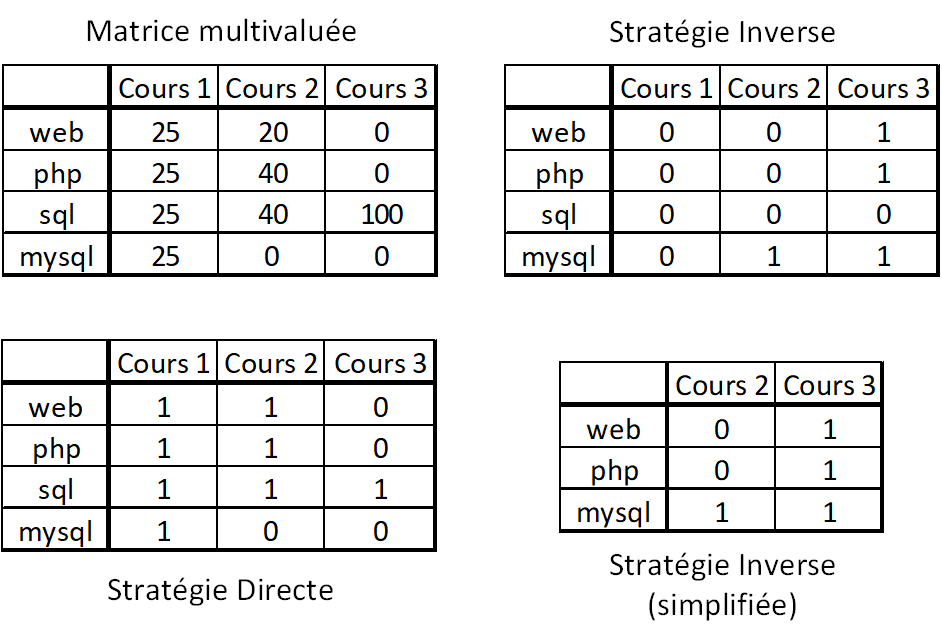
\includegraphics[scale=1]{2-Etat-de-l'Art/images/ACF/Strategies/exemple_strategies_simples.png}
\caption{Exemple d'application des stratégies directe et inverse}
\label{figure:2-S2-Exemple-Strategies-Simples}
\end{figure}
%\end{figure*} % Figure flottante
% To use it : fig~\ref{label}

\bigskip

Trois autres stratégies prenant en compte la pondération sont aussi présentées dans~\cite{jaffal2015refinement}\cite{jaffal2019aide}.
Celles-ci se basent sur la prise en compte de \textit{l'intensité de la relation entre chaque objet et chaque attribut, via le calcul d'une valeur de fréquence}~\cite{jaffal2019aide}.
Deux seuils sont fixés par un $ \beta \in [0, 1] $.
Les seuils sont équidistants de la valeur $ 0,5 $ (indiquée par la ligne en pointillés rouges) et s'en éloignent au fur et à mesure que $ \beta $ augmente, comme illustré sur la figure~\ref{figure:2-S2-Strategies-Exemple-Seuils}.
Ces seuils permettent de découper l'espace entre $ 0 $ et $ 1 $ en trois parties : les valeurs de fréquences hautes (au dessus du \textit{seuil haut}) associées à la \textit{stratégie à haute dépendance}, les valeurs de fréquences basses (en dessous du \textit{seuil bas}) associées à la \textit{stratégie à faible dépendance}, et les valeurs de fréquences moyennes (entre les \textit{seuil haut} et \textit{seuil bas}) associées à la \textit{stratégie à dépendance moyenne}.

La figure~\ref{figure:2-S2-Strategies-Exemple-Trois-Parties} présente plusieurs exemples suivant les valeurs de $ \beta $.
On notera que lorsque $ \beta $ vaut $ 0 $, il n'y a qu'un seuil à $ 0,5 $ découpant l'espace en seulement deux parties (les valeurs à fréquences hautes et basses), et inversement, lorsque $ \beta $ vaut $ 1 $, les deux seuils sont à $ 0 $ et $ 1 $ découpant l'espace en seulement une partie (les valeurs à fréquences moyennes).

%\begin{figure*} % Figure flottante
\begin{figure}[ht]
\centering
\centerline{
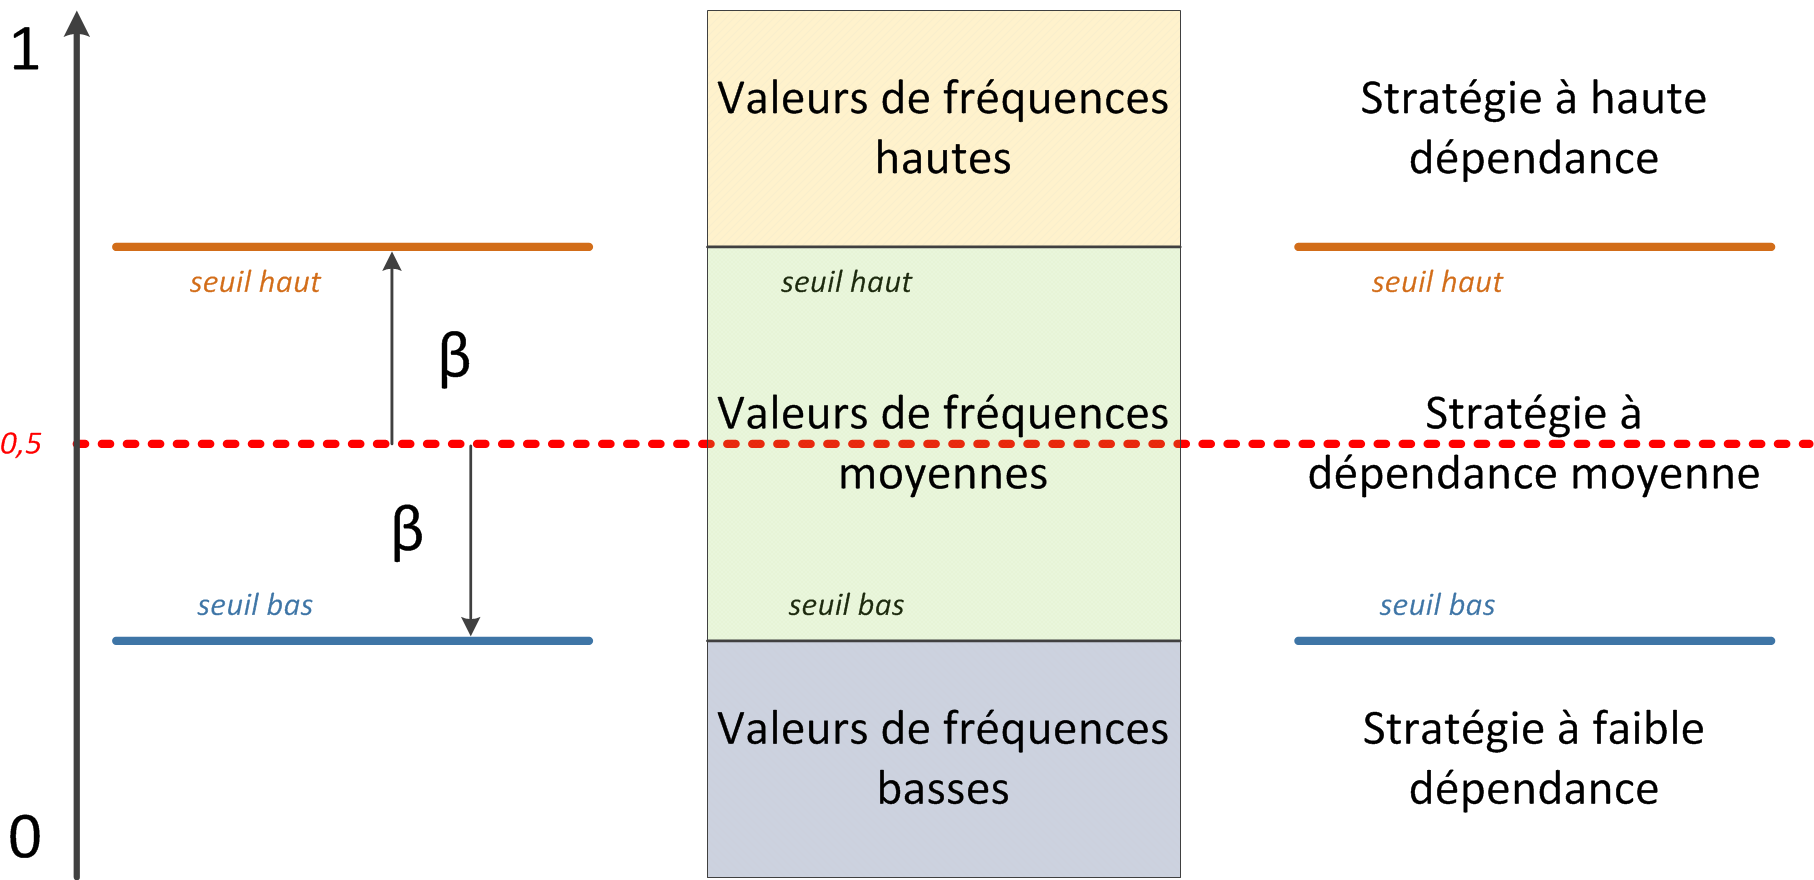
\includegraphics[scale=0.65]{2-Etat-de-l'Art/images/ACF/Strategies/explication_strategies_seuils_beta.png}
}
\caption{Les deux seuils générés par $ \beta $ découpent l'espace en trois parties}
\label{figure:2-S2-Strategies-Exemple-Seuils}
\end{figure}
%\end{figure*} % Figure flottante
% To use it : fig~\ref{label}

%\begin{figure*} % Figure flottante
\begin{figure}[ht]
\centering
%\includegraphics[width=3in]{images/VerySmallModels_text.png}
%%\includegraphics[scale=0.6]{images/VerySmallModels_text.png}
\centerline{  % FORCE FIGURE OUTSIDE THE MARGIN !!! BUT STILL CENTERING !!!
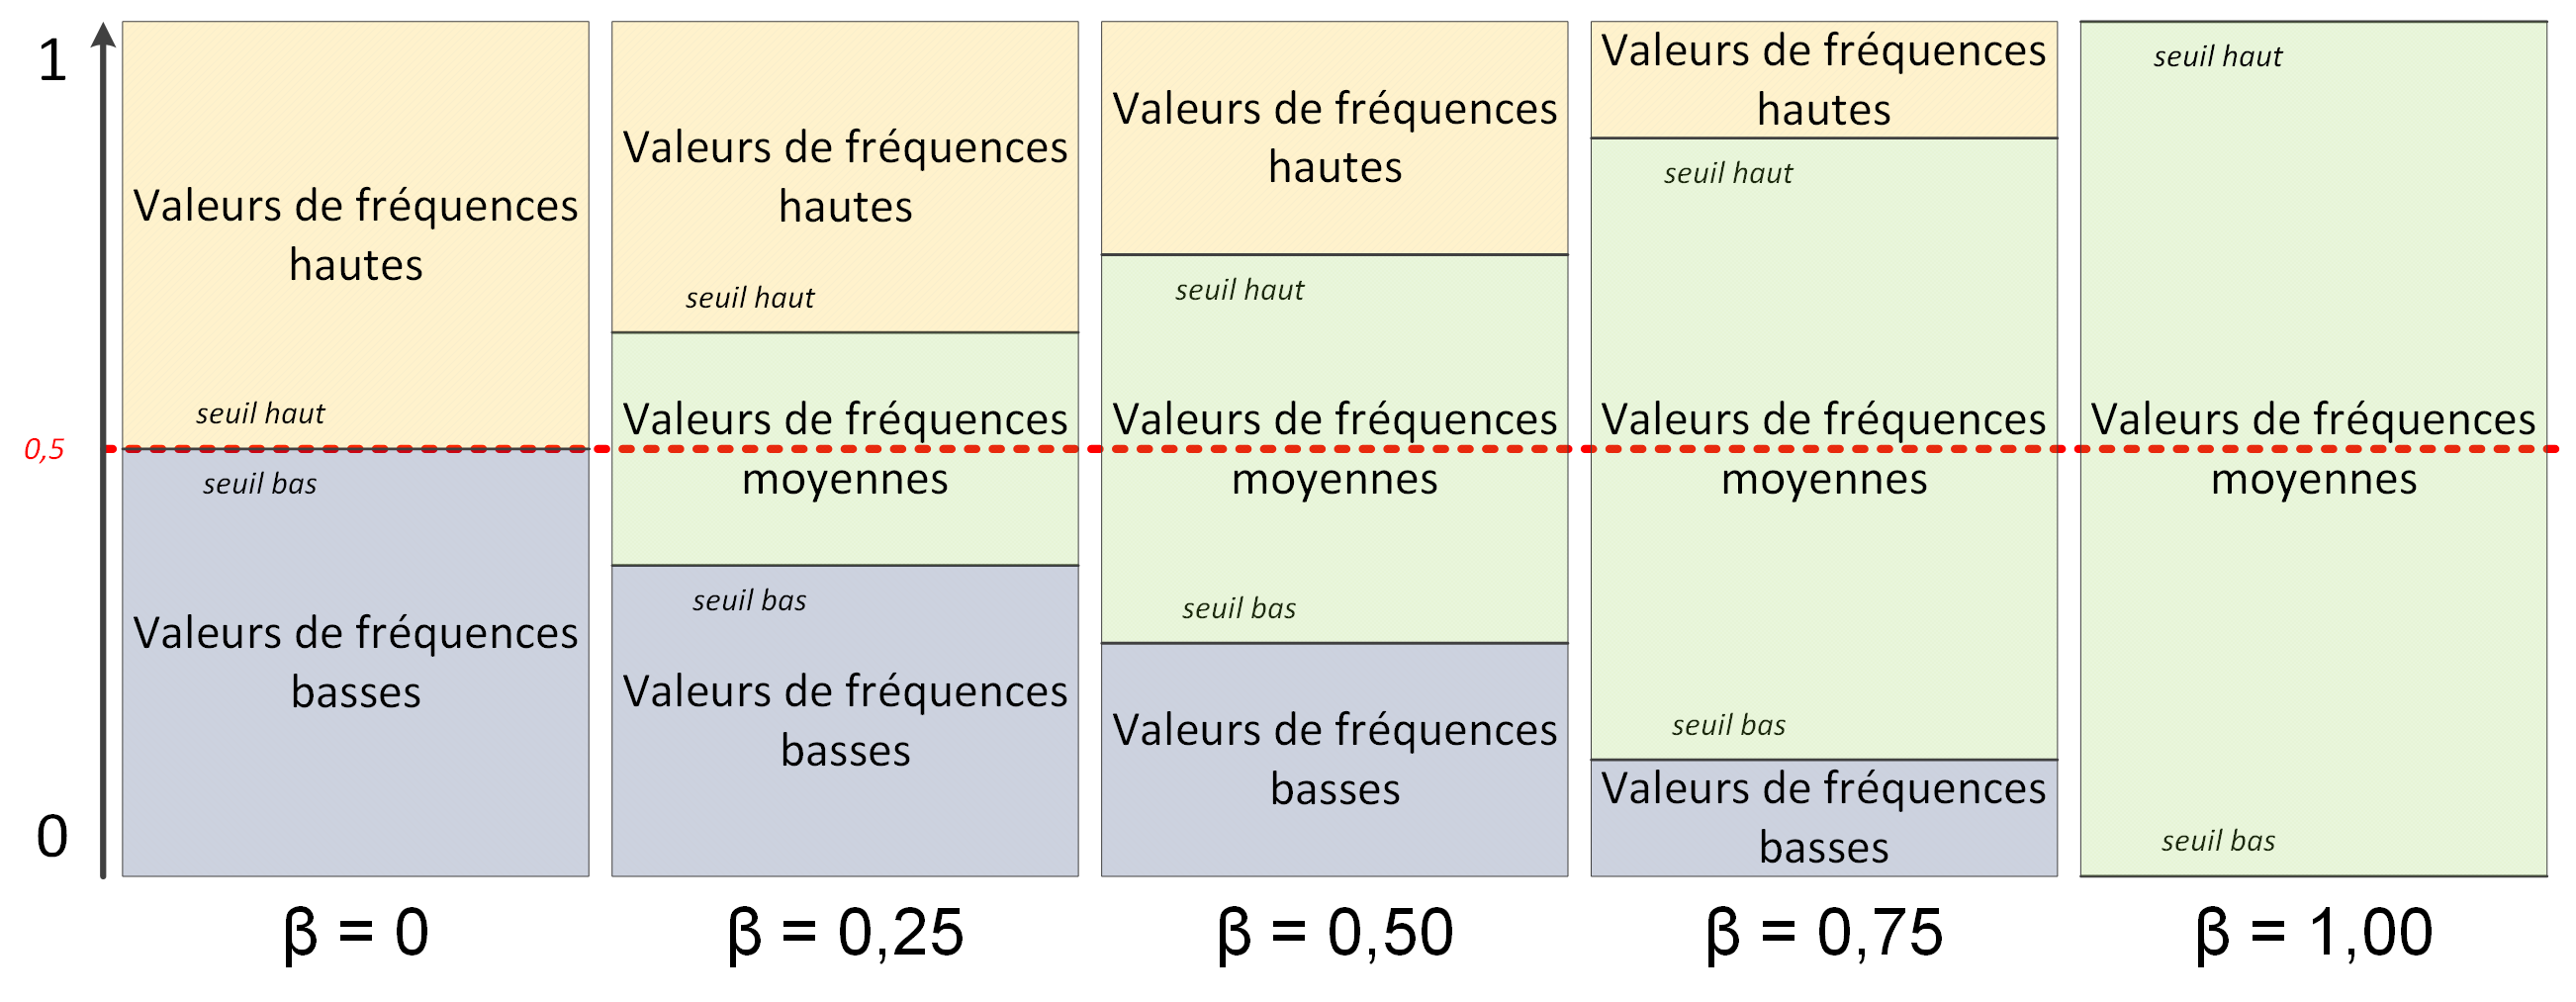
\includegraphics[scale=0.6]{2-Etat-de-l'Art/images/ACF/Strategies/explication_strategies_trois_parties.png}
}
\caption{Différentes valeurs de $ \beta $ séparent l'espace en plusieurs parties}
\label{figure:2-S2-Strategies-Exemple-Trois-Parties}
\end{figure}
%\end{figure*} % Figure flottante
% To use it : fig~\ref{label}

\bigskip

Selon le $ \beta $ choisi, les seuils vont se fixer pour permettre de délimiter les bornes des valeurs de fréquences requises pour chaque stratégie.
Ensuite, la formule~\eqref{equation:2-S2-Strategies-Frequence} permet d'obtenir la valeur de fréquence pour chaque proportion d'occurrences d'un terme dans un document de la matrice fournie.
La valeur de fréquence ainsi obtenue est transformée en $ 0 $ ou $ 1 $ selon son positionnement entre les seuils (et donc par rapport à la stratégie sélectionnée).
Les seuils hauts et bas sont positionnés en suivant les formules~\eqref{equation:2-S2-Strategies-Seuil-Haut} et~\eqref{equation:2-S2-Strategies-Seuil-Bas}.
La matrice multivaluée est ainsi transformée en matrice binaire qui peut être utilisée comme un \textit{contexte formel} par la suite.
Afin de générer une matrice binaire, il faut donc fixer un $ \beta $ et sélectionner une stratégie parmi les suivantes :
\begin{itemize}
\item La \textit{stratégie à haute dépendance} contient les termes dont la valeur de fréquence est supérieure au seuil haut.
Il s'agit des termes qui apparaissent les plus fréquemment dans l'ensemble des documents.
\item La \textit{stratégie à faible dépendance} contient les termes dont la valeur de fréquence est inférieure au seuil bas.
Il s'agit des termes qui apparaissent les moins fréquemment dans l'ensemble des documents.
\item La \textit{stratégie à dépendance moyenne} contient les termes dont la valeur de fréquence est inférieure au seuil haut tout en étant supérieure au seuil bas.
Il s'agit des termes qui apparaissent ni trop fréquemment ni trop rarement dans l'ensemble des documents.
\end{itemize}

\begin{equation}
\text{\textit{fréquence}}(T, D) = \frac{\text{\textit{Nb d'occurrences du terme T dans le document D}}}{\text{\textit{Nb d'occurrences du terme T dans tous les documents}}}
\label{equation:2-S2-Strategies-Frequence}
\end{equation}

\begin{equation}
\text{\textit{seuil haut}} = \text{\textit{Moyenne des fréquences}} + \beta \times \text{\textit{Écart type des fréquences}}
\label{equation:2-S2-Strategies-Seuil-Haut}
\end{equation}

\begin{equation}
\text{\textit{seuil bas}} = \text{\textit{Moyenne des fréquences}} - \beta \times \text{\textit{Écart type des fréquences}}
\label{equation:2-S2-Strategies-Seuil-Bas}
\end{equation}

\bigskip

La figure~\ref{figure:2-S2-Strategies-Exemple-Beta} illustre ces trois stratégies avec un $ \beta $ fixé à 0,50.
On remarque que les valeurs non nulles de chaque ligne sont distribuées dans chacune des stratégies : \textit{web} et \textit{php} voient leurs deux valeurs non nulles distribuées dans les stratégies basses et hautes, \textit{sql} voit ses trois valeurs distribuées dans toutes les stratégies, tandis que \textit{mysql} a son unique valeur non nulle rattachée à la stratégie moyenne.

%\begin{figure*} % Figure flottante
\begin{figure}[ht]
\centering
\centerline{  % FORCE FIGURE OUTSIDE THE MARGIN !!! BUT STILL CENTERING !!!
% scale = 0.6
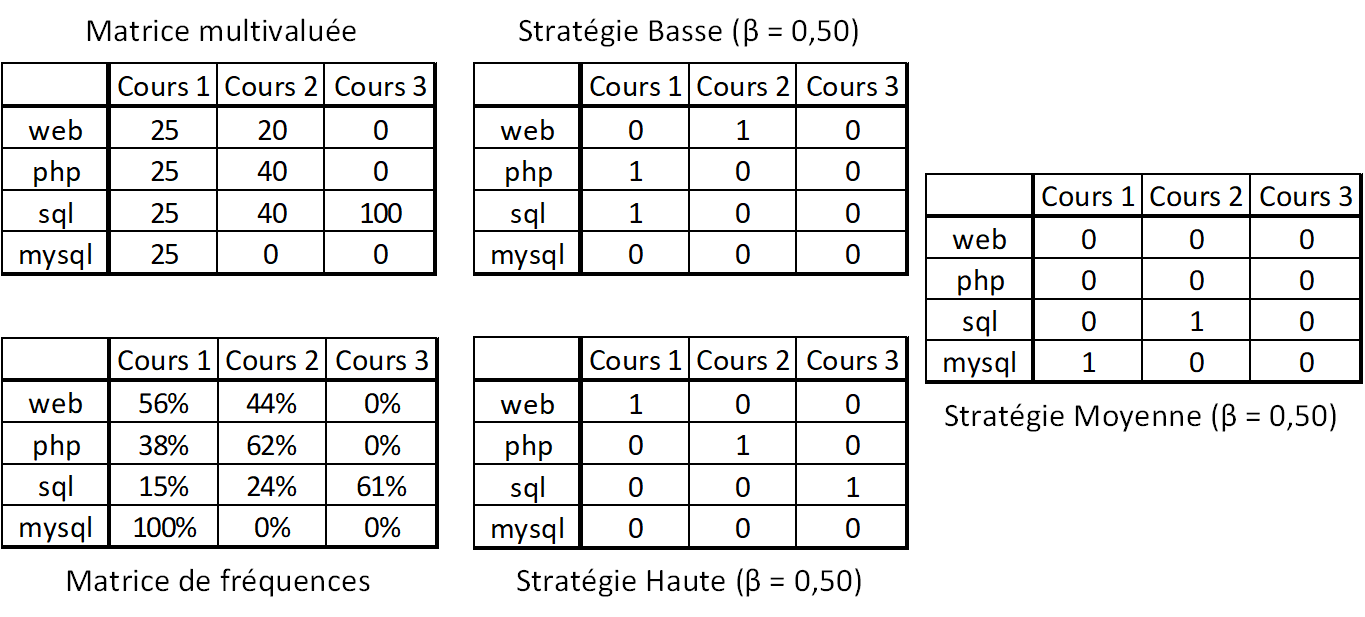
\includegraphics[scale=1]{2-Etat-de-l'Art/images/ACF/Strategies/exemple_strategies_beta=0.50.png}
}
\caption{Exemple d'application des stratégies complexes avec un $ \beta = 0,50 $}
\label{figure:2-S2-Strategies-Exemple-Beta}
\end{figure}
%\end{figure*} % Figure flottante
% To use it : fig~\ref{label}



\bigskip
%\newpage % esthétique

%%%%%%%%%%%%%%%%%%%%%%%%%%%%%%%%%%%%%%%%%%%%
%\clearpage % Clean for pictures and tables %
%\newpage   % Clean for pictures and tables %
%%%%%%%%%%%%%%%%%%%%%%%%%%%%%%%%%%%%%%%%%%%%

\subsubsection{Construction du treillis de Galois (PII.1.d) :}
\label{subsubsection:Contexte:ACF-ConstructionTreillis}

Le \textit{contexte formel} généré avec les stratégies de binarisation contient maintenant des termes liés à des documents par des $ 0 $ et des $ 1 $.
Il peut maintenant être transformé en un \textit{treillis de Galois} pour en extraire des \textit{concepts formels} qui serviront de \textit{fragments} (de cas passés) réutilisables.

\bigskip

La construction d'un treillis de Galois depuis un contexte formel peut se réaliser avec plusieurs algorithmes~\cite{messai2009analyse}.
Chaque n\oe{}ud du treillis correspond à un \textit{concept formel}.
Un \textit{concept formel} contient le maximum d'objets partageant un maximum d'attributs communs, c'est-à-dire que le maximum de termes sont rassemblés selon le maximum de documents auxquels ils sont liés.
La figure~\ref{figure:2-S2-Treillis-Construction-Treillis} illustre le treillis de Galois issu d'un contexte formel (une version simplifiée du contexte formel est présente, afin de mieux observer les résultats sur le treillis).
Les concepts formels aux deux extrémités haute et basse du treillis contiennent respectivement l'ensemble des objets (avec éventuellement le(s) attribut(s) commun(s) à tous les objets) et l'ensemble des attributs (avec éventuellement le(s) objet(s) commun(s) à tous les attributs).

%\begin{figure*} % Figure flottante
\begin{figure}[ht]
\centering
\centerline{  % FORCE FIGURE OUTSIDE THE MARGIN !!! BUT STILL CENTERING !!!
% scale = 0.8
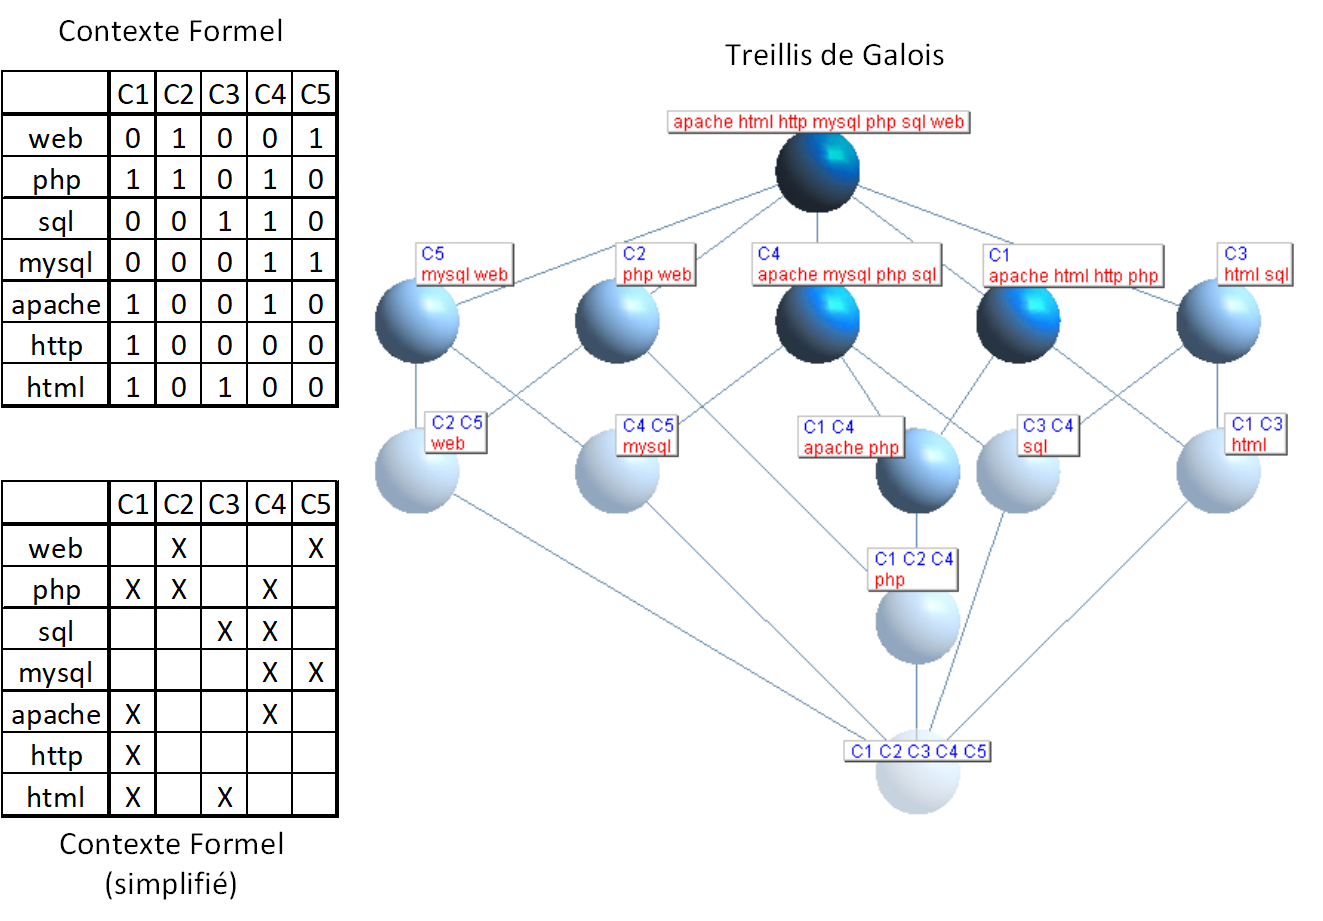
\includegraphics[scale=1]{2-Etat-de-l'Art/images/ACF/Treillis/exemple_treillis_ExampleMediumMatrix-S-B-B-0.00.png}
}
\caption{Contexte formel et son treillis de Galois}
\label{figure:2-S2-Treillis-Construction-Treillis}
\end{figure}
%\end{figure*} % Figure flottante
% To use it : fig~\ref{label}

\bigskip

Dans l'exemple, nous retrouvons donc l'ensemble des termes du contexte formel (qui ne partagent aucun document commun) dans le concept formel du haut, et l'ensemble des documents (qui ne partagent aucun terme commun) dans le concept formel du bas.
En partant du concept formel contenant tous les objets, chaque attribut non nul du contexte formel est progressivement ajouté pour former le plus grand sous-ensemble d'objets.
Chaque niveau du treillis introduit ainsi un attribut supplémentaire (certains niveaux peuvent être vides).
Dans notre exemple, nous voyons au niveau 0 l'ensemble des termes "\textit{apache}", "\textit{html}", "\textit{http}", "\textit{mysql}", "\textit{php}", "\textit{sql}", et "\textit{web}", puis au niveau 1, un document est ajouté à chaque concept formel pour former le sous-ensemble le plus grand de termes partageant cet attribut commun : "\textit{apache}", "\textit{mysql}", "\textit{php}", et "\textit{sql}" ont le document "\textit{C4}" en commun, mais "\textit{apache}", "\textit{html}", "\textit{http}", et "\textit{php}" ont le document "\textit{C1}" en commun.
En niveau 2, un sous-ensemble plus restreint de termes possède deux documents en commun : "\textit{apache}" et "\textit{php}" partagent les documents "\textit{C1}" et "\textit{C4}".
Ensuite, au niveau 3, seul le terme "\textit{php}" est partagé par trois documents "\textit{C1}", "\textit{C2}", et "\textit{C4}".
Finalement, au niveau 4, les cinq documents du contexte formel sont réunis en un concept formel sans aucun terme.

%\begin{figure*} % Figure flottante
\begin{figure}[ht]
\centering
\centerline{  % FORCE FIGURE OUTSIDE THE MARGIN !!! BUT STILL CENTERING !!!
% scale = 0.7
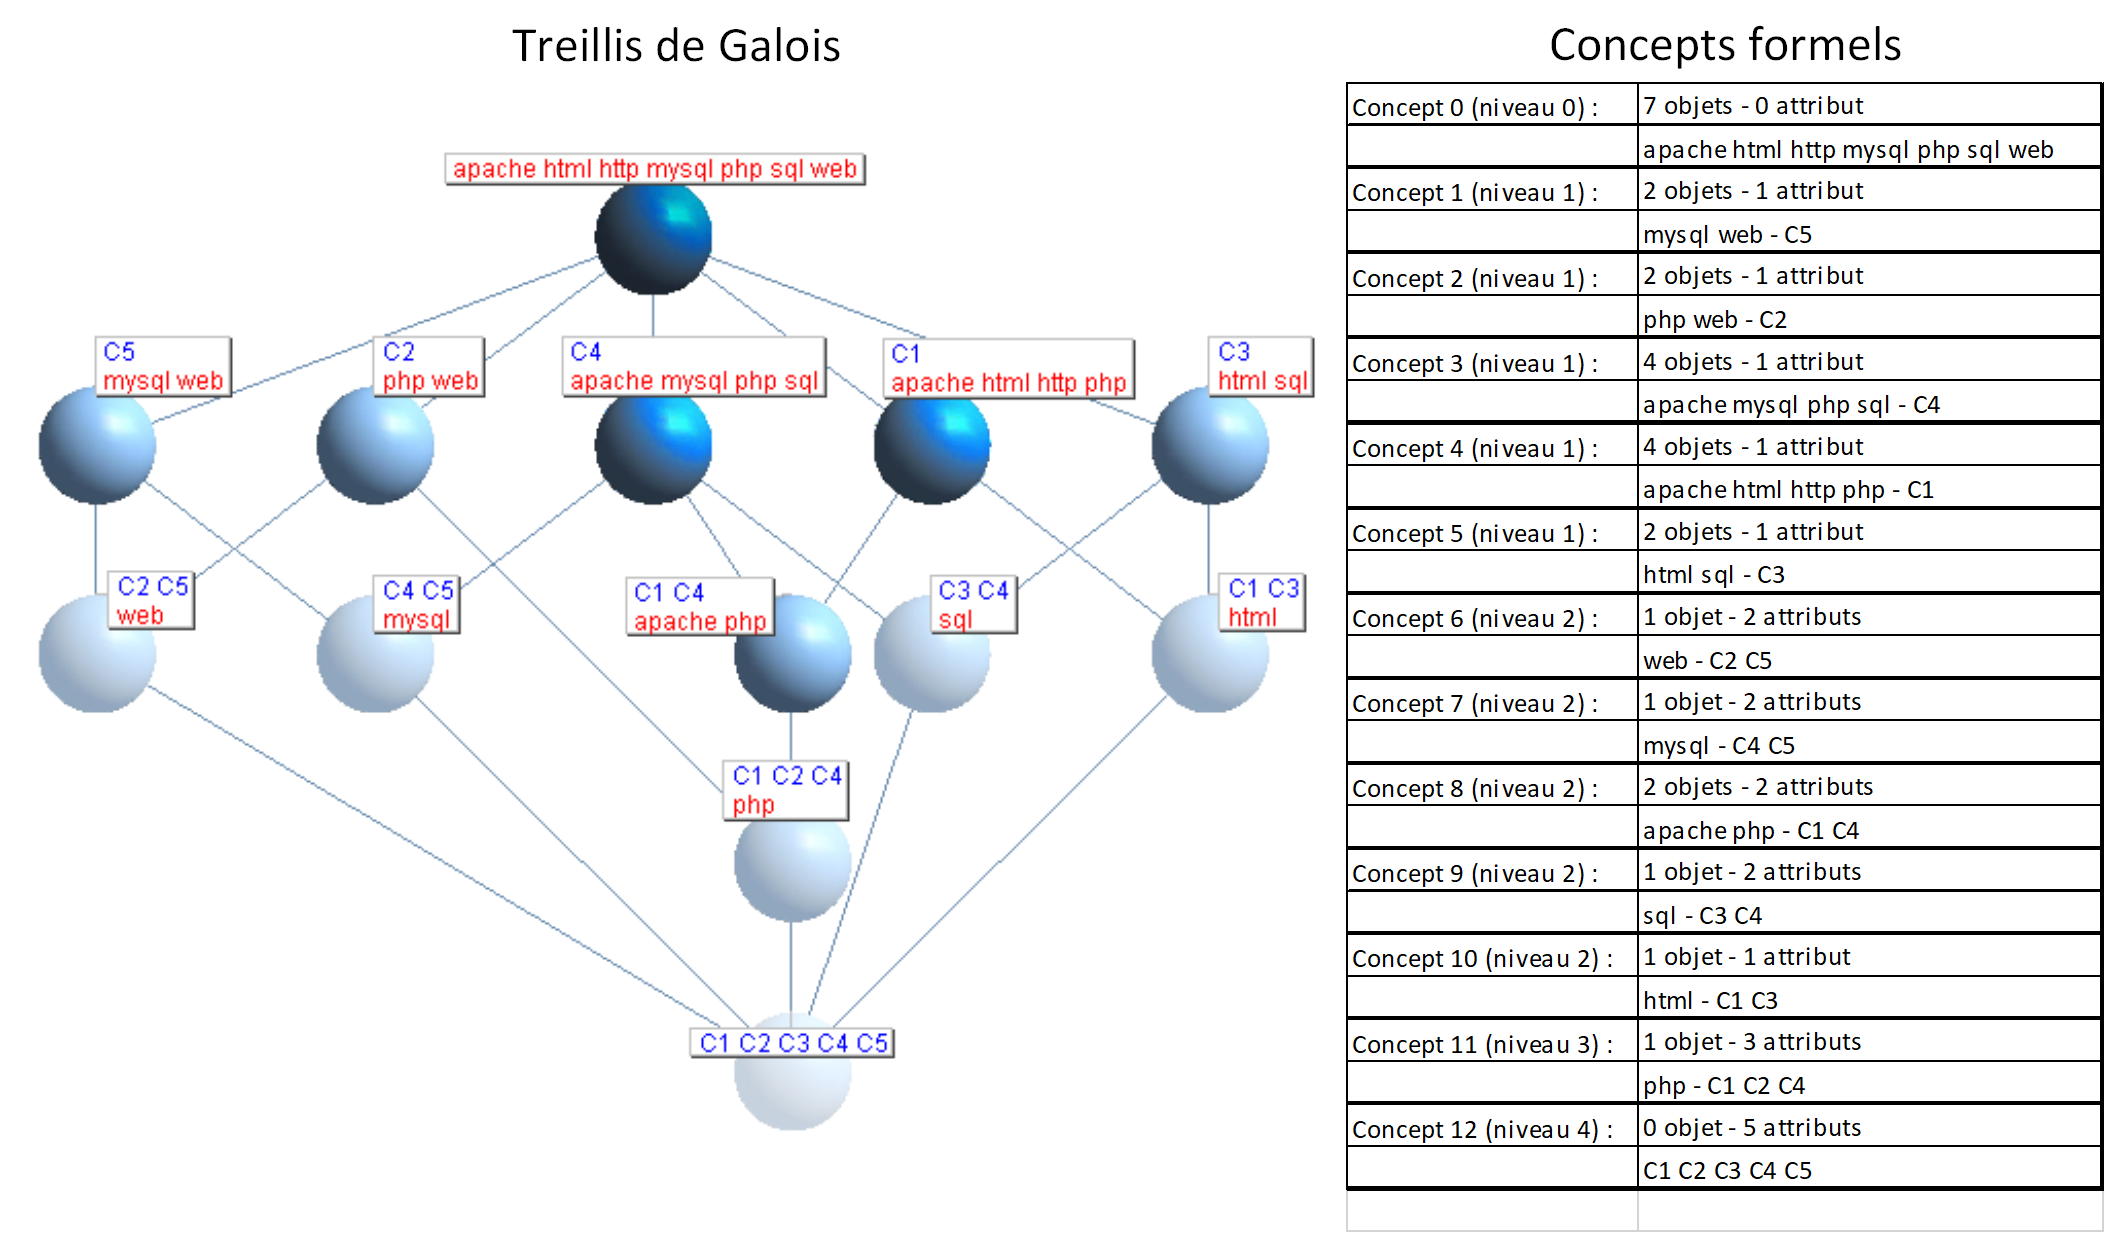
\includegraphics[scale=0.7]{2-Etat-de-l'Art/images/ACF/Treillis/exemple_treillis-concepts_ExampleMediumMatrix-S-B-B-0.00.png}
}
\caption{Treillis de Galois et ses concepts formels}
\label{figure:2-S2-Treillis-Concepts}
\end{figure}
%\end{figure*} % Figure flottante
% To use it : fig~\ref{label}

\bigskip

Dans l'exemple précédent, treize concepts formels ont été générés à partir du contexte formel pour construire le treillis de Galois (ceux-ci sont explicités sur la figure~\ref{figure:2-S2-Treillis-Concepts}).
Ces concepts formels regroupent donc des termes et les documents auxquels ils sont rattachés, c'est-à-dire, suite aux stratégies de binarisation, chaque concept formel rassemble des termes qui apparaissent ensemble dans un ou plusieurs documents selon leurs fréquences d'apparitions communes.
Les concepts formels ainsi formés permettent de manipuler des informations plus abstraites grâce à la combinaison de termes et documents engendrée par le treillis de Galois.


%\bigskip
\newpage % esthétique

%%%%%%%%%%%%%%%%%%%%%%%%%%%%%%%%%%%%%%%%%%%%
%\clearpage % Clean for pictures and tables %
%\newpage   % Clean for pictures and tables %
%%%%%%%%%%%%%%%%%%%%%%%%%%%%%%%%%%%%%%%%%%%%

\subsubsection{Calcul des métriques du treillis (PII.1.e) :}
\label{subsubsection:Contexte:ACF-MetriquesTreillis}

L'ACF permet de calculer de nombreuses métriques sur le treillis généré~\cite{babin2012approximating}\cite{jaffal2019aide} : stabilité des concepts, poids conceptuel des objets (respectivement des attributs), similarité conceptuelle des objets (respectivement des attributs), impact mutuel absolu entre un objet et un attribut, impact mutuel relatif entre un objet et un attribut, et beaucoup d'autres.
Dans le cas de la méthode CREA, nous nous concentrons particulièrement sur l'impact mutuel relatif~\cite{jaffal2019aide} qui permet de générer des graphiques utiles pour évaluer la qualité des données (présentés en sous-section~\ref{subsection:CREA:PII.2-GrapheImpactMutuel}), ainsi que la similarité conceptuelle des objets~\cite{jaffal2019aide} nécessaire pour d'autres traitements ultérieurs (notamment lors du regroupement des termes présenté en sous-section~\ref{subsection:CREA:PII.3-ConstructionClusters}).

\bigskip

\paragraph{Similarité Conceptuelle entre deux objets :}
\label{mystep:Contexte:ACF-MetriquesTreillis-SimilariteConceptuelle}

La \textit{similarité conceptuelle} permet de comparer deux objets (respectivement attributs) en tenant compte de leurs présences dans l'ensemble du treillis.
C'est-à-dire, la métrique correspond à la fréquence d'apparition des objets dans les concepts formels du treillis.
La formule calculant la similarité conceptuelle entre deux objets est la suivante :

\begin{equation}
\text{\textit{Similarité conceptuelle}}(O_{i}, O_{j}) = \frac{\text{\textit{Nombre de concepts contenant} } O_{i} \text{ \textbf{et} } O_{j}}{\text{\textit{Nombre de concepts contenant} } O_{i} \text{ \textbf{ou} } O_{j}}
\label{equation:2-S2-Metriques-SimilariteConceptuelle}
\end{equation}

La similarité conceptuelle étant un rapport, elle prend des valeurs entre $ 0 $ et $ 1 $.
La valeur maximale $ 1 $ indique que les deux objets (respectivement attributs) sont toujours présents ensemble dans les mêmes concepts formels du treillis, c'est-à-dire qu'il n'existe aucun concept formel ne contenant que l'un des deux objets (respectivement attributs), ou encore qu'ils partagent exactement les mêmes attributs (respectivement objets).
L'exemple en figure~\ref{figure:2-S2-Metriques-SimilariteConceptuelle-Exemple} illustre le calcul de la similarité entre deux objets.

\bigskip

Il est possible de générer un tableau regroupant les similarités conceptuelles entre tous les objets (respectivement attributs) d'un treillis, ce qui a pour conséquence de former une \textit{matrice de similarité conceptuelle}.
La figure~\ref{figure:2-S2-Metriques-SimilariteConceptuelle-Matrice} illustre une matrice de similarité conceptuelle regroupant les similarités conceptuelles de tous les objets d'un treillis.

\bigskip

Dans le cadre de la méthode CREA, la matrice de similarité conceptuelle est une donnée d'entrée aux méthodes de \textit{clustering} abordées plus tard en sous-section~\ref{subsection:CREA:PII.3-ConstructionClusters}.

\bigskip

\vfill
\hspace{0pt}

%%%%%%%%%%%%%
%% ESTHETIQUE

\begin{figure}[htb!]
\centering
\centerline{  % FORCE FIGURE OUTSIDE THE MARGIN !!! BUT STILL CENTERING !!!
% scale = 0.85
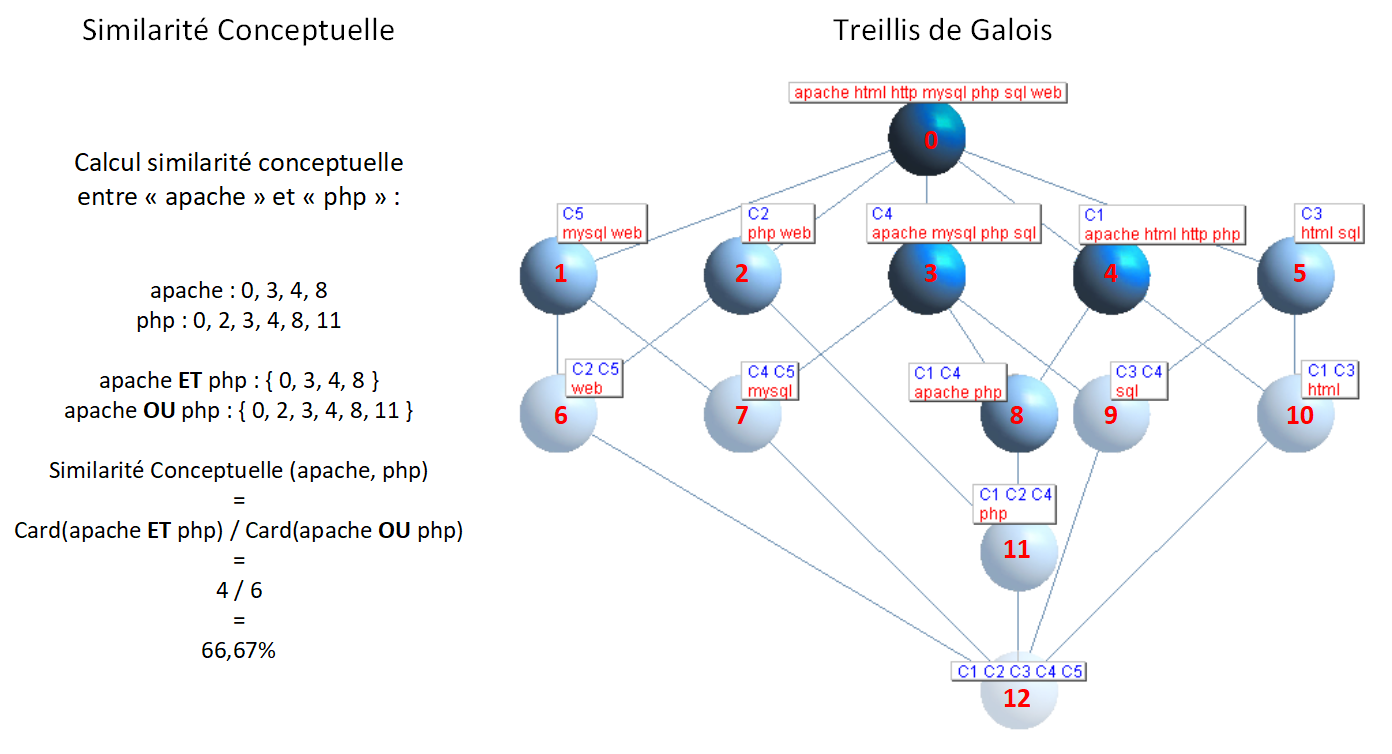
\includegraphics[scale=1]{2-Etat-de-l'Art/images/ACF/Metriques/exemple_similarite-conceptuelle_calcul.png}
}
\caption{Calcul de la similarité conceptuelle entre deux objets}
\label{figure:2-S2-Metriques-SimilariteConceptuelle-Exemple}
\end{figure}

\hspace{0pt}
\vfill

\newpage % esthétique

\begin{figure}[htb!]
\centering
%\includegraphics[width=3in]{images/VerySmallModels_text.png}
%%\includegraphics[scale=0.6]{images/VerySmallModels_text.png}
\centerline{  % FORCE FIGURE OUTSIDE THE MARGIN !!! BUT STILL CENTERING !!!
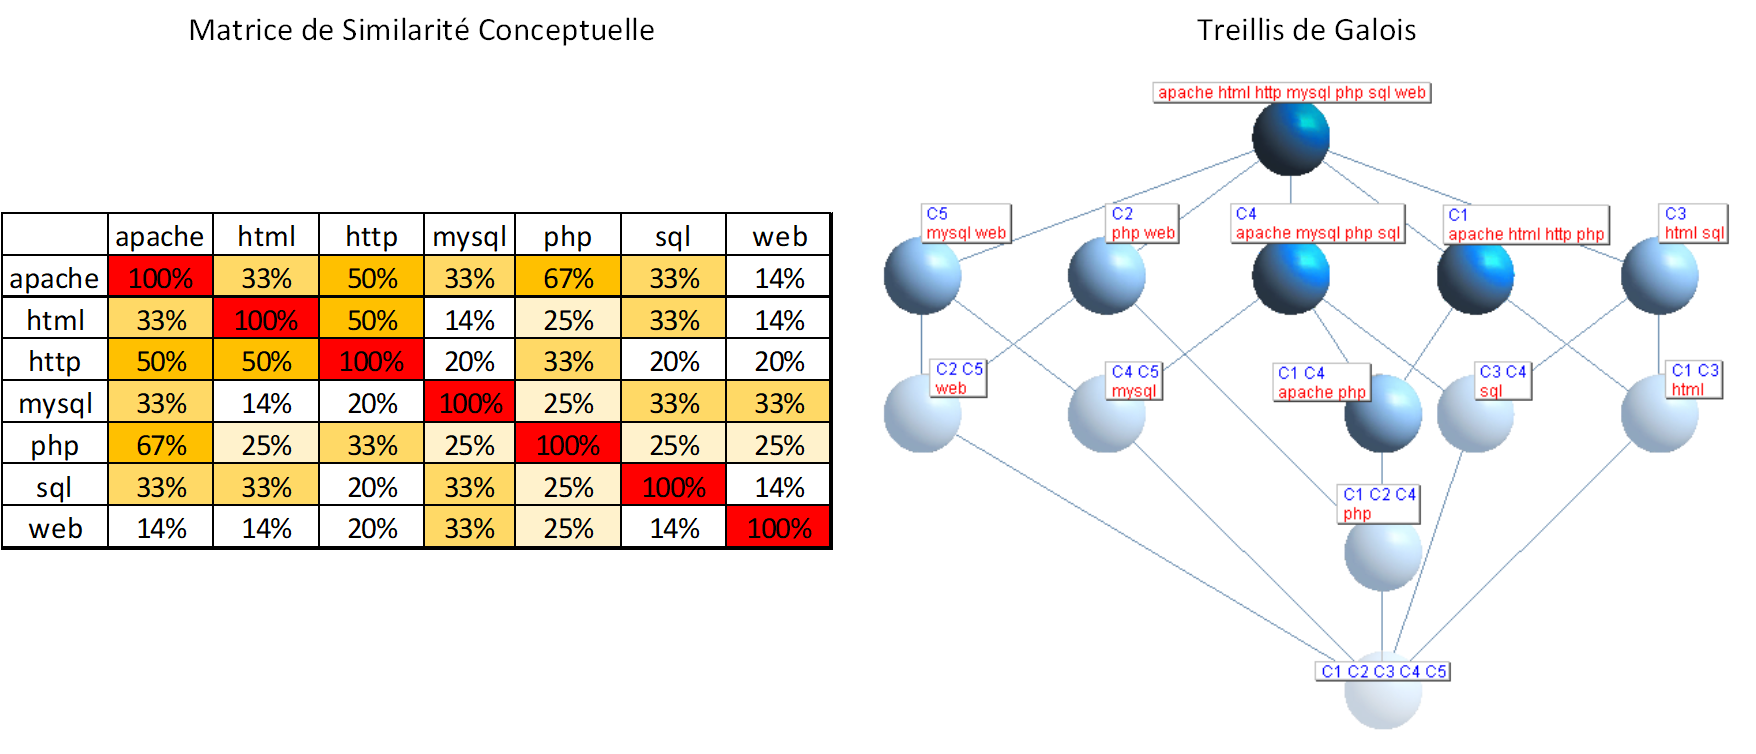
\includegraphics[scale=0.85]{2-Etat-de-l'Art/images/ACF/Metriques/exemple_similarite-conceptuelle_matrice.png}
}
\caption{Matrice de similarité conceptuelle}
\label{figure:2-S2-Metriques-SimilariteConceptuelle-Matrice}
\end{figure}

%% FIN ESTHETIQUE
%%%%%%%%%%%%%

\bigskip

%\clearpage % Clean for pictures and tables %


\paragraph{Impact mutuel entre un objet et un attribut :}
\label{mystep:Contexte:ACF-MetriquesTreillis-ImpactMutuel}

L'\textit{impact mutuel} analyse la "\textit{force de la relation entre un objet O$_{i}$ et un attribut A$_{j}$ en fonction des concepts formels qui les associent}"~\cite{jaffal2019aide}.
Il est défini à partir de l'équation suivante :

\bigskip

\begin{equation}
\text{\textit{Impact mutuel}}(O_{i}, A_{j}) = \frac{\text{\textit{Nombre de concepts contenant} } O_{i} \text{ \textbf{et} } A_{j}}{\text{\textit{Nombre de concepts contenant} } O_{i} \text{ \textbf{ou} } A_{j}}
\label{equation:2-S2-Metriques-ImpactMutuel}
\end{equation}


\bigskip % esthétique

L'impact mutuel étant un rapport, il prend des valeurs entre $ 0 $ et $ 1 $.
Plus la valeur de l'impact mutuel est élevée, plus l'attribut caractérise l'objet parmi tous les autres, et réciproquement : plus l'objet se définit particulièrement grâce à cet attribut.
En d'autres termes, un impact mutuel proche de $ 1 $ implique que l'attribut apparait quasiment uniquement avec cet objet, et réciproquement, l'objet n'a quasiment pas d'autre attribut.
À l'inverse, un impact mutuel proche de $ 0 $, mais non nul, implique que l'attribut est partagé par énormément d'objets, et réciproquement, que l'objet utilise quasiment tous les attributs existants.
L'exemple en figure~\ref{figure:2-S2-Metriques-ImpactMutuel-Exemple} illustre le calcul de l'impact mutuel entre un objet et un attribut.

%\begin{figure*} % Figure flottante
\begin{figure}[htb!]
\centering
%\includegraphics[width=3in]{images/VerySmallModels_text.png}
%%\includegraphics[scale=0.6]{images/VerySmallModels_text.png}
\centerline{  % FORCE FIGURE OUTSIDE THE MARGIN !!! BUT STILL CENTERING !!!
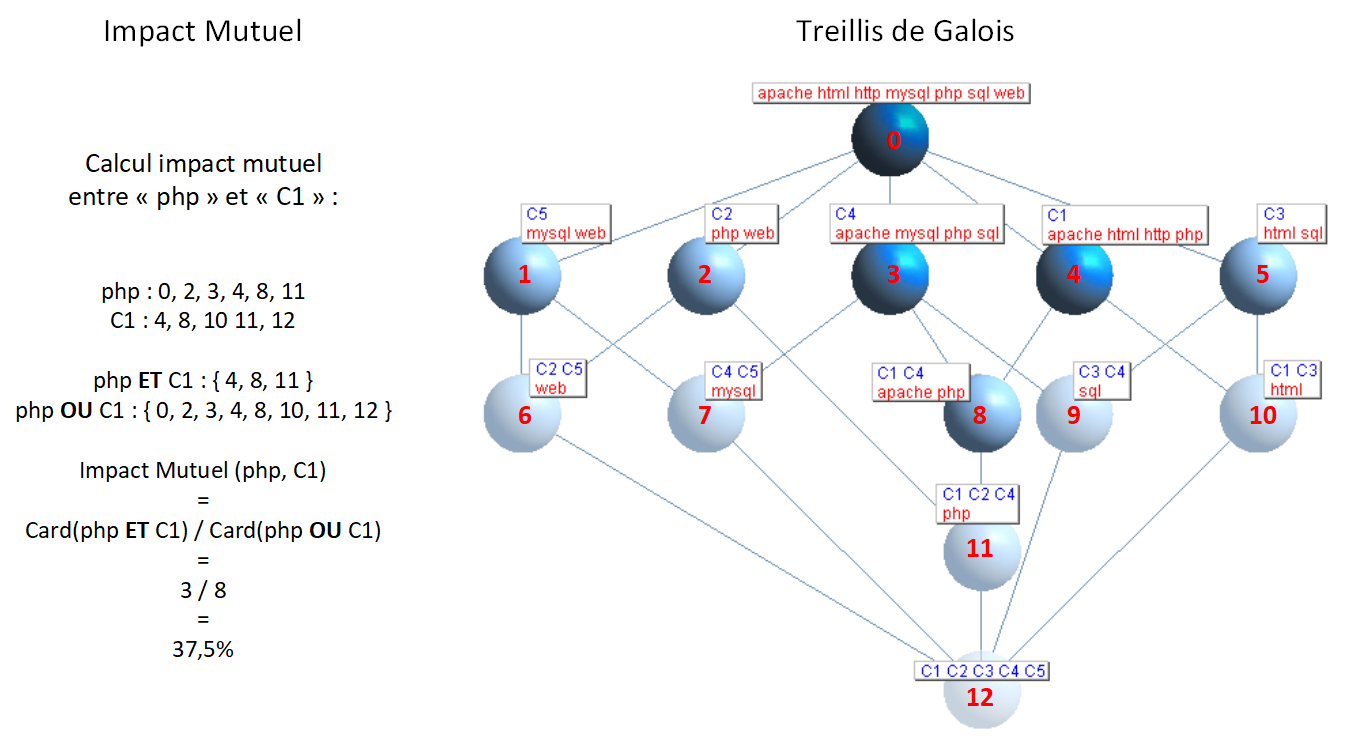
\includegraphics[scale=1]{2-Etat-de-l'Art/images/ACF/Metriques/exemple_impact-mutuel_calcul.png}
}
\caption{Calcul de l'impact mutuel entre un objet et un attribut}
\label{figure:2-S2-Metriques-ImpactMutuel-Exemple}
\end{figure}
%\end{figure*} % Figure flottante
% To use it : fig~\ref{label}

Le tableau regroupant les impacts mutuels entre tous les objets et attributs d'un treillis s'appelle une \textit{matrice d'impact mutuel}.
La figure~\ref{figure:2-S2-Metriques-ImpactMutuel-Matrice} illustre une matrice d'impact mutuel regroupant les impacts mutuels entre chaque objet et chaque attribut d'un treillis.

%\begin{figure*} % Figure flottante
\begin{figure}[htb!]
\centering
\centerline{  % FORCE FIGURE OUTSIDE THE MARGIN !!! BUT STILL CENTERING !!!
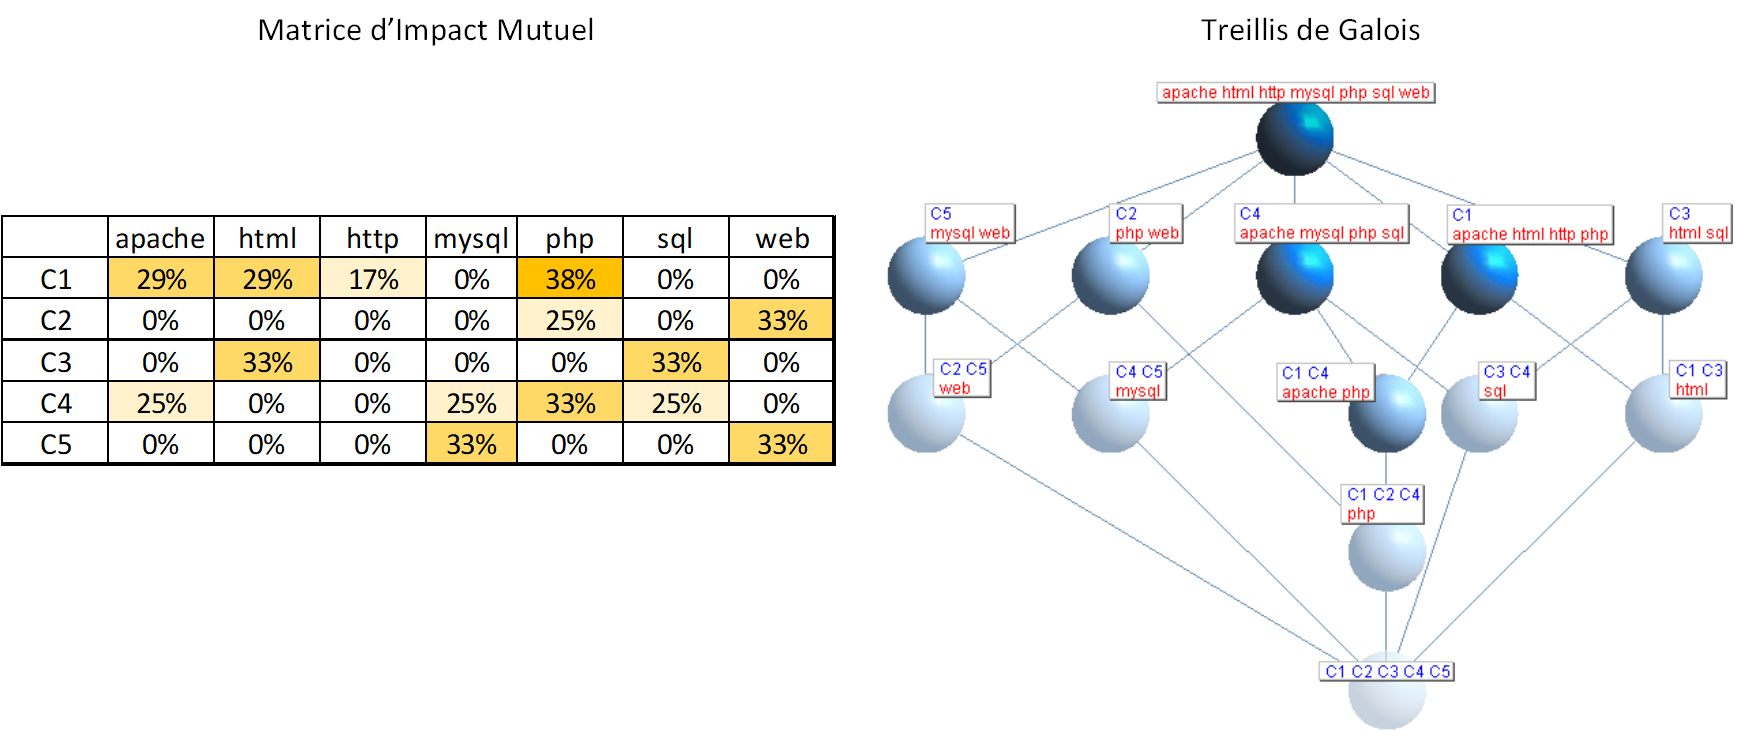
\includegraphics[scale=0.8]{2-Etat-de-l'Art/images/ACF/Metriques/exemple_impact-mutuel_matrice.png}
}
\caption{Matrice d'impact mutuel}
\label{figure:2-S2-Metriques-ImpactMutuel-Matrice}
\end{figure}
%\end{figure*} % Figure flottante
% To use it : fig~\ref{label}

\bigskip

La matrice d'impact mutuel permet de générer un \textit{graphe d'impact mutuel}.
Le graphe d'impact mutuel a la particularité d'être bi-parti, en proposant des n\oe{}uds de la classe des objets, et des n\oe{}uds de la classe des attributs.
Dans le cadre de la méthode CREA, ce graphe permet de déterminer visuellement deux informations importantes : les termes les plus représentatifs du corpus de documents rassemblés ; la pertinence des documents dans le contexte ainsi formé.
La figure~\ref{figure:2-S2-Metriques-ImpactMutuel-Graphe} illustre le graphe d'impact mutuel et fait un agrandissement de l'ensemble central où le document \textit{C1} apparait parmi des termes.

%\begin{figure*} % Figure flottante
\begin{figure}[htb!]
\centering
\centerline{  % FORCE FIGURE OUTSIDE THE MARGIN !!! BUT STILL CENTERING !!!
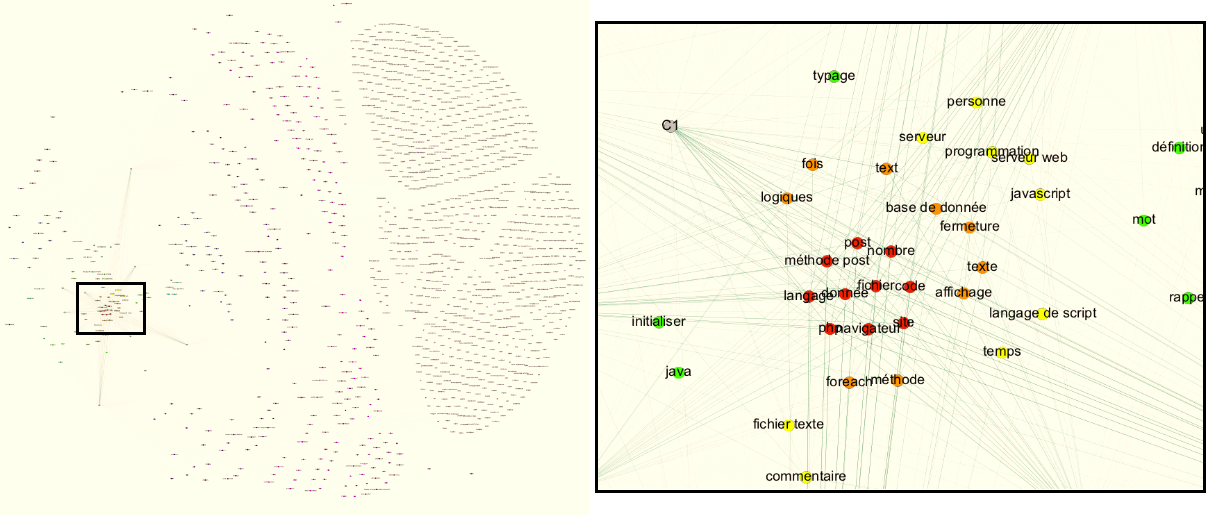
\includegraphics[scale=0.6]{2-Etat-de-l'Art/images/ACF/Metriques/exemple_graphe.png}
}
\caption{Graphe d'impact mutuel (généré avec Gephi en utilisant la spatialisation \textit{Force Atlas} et la coloration par \textit{partition} selon le \textit{degré}) et agrandissement de la communauté centrale}
\label{figure:2-S2-Metriques-ImpactMutuel-Graphe}
\end{figure}
%\end{figure*} % Figure flottante
% To use it : fig~\ref{label}

\bigskip

Typiquement, un ou des documents excentrés et avec peu de liens peuvent être considérés comme peu pertinents, voire comme du \textit{bruit} d'un point de vue statistique.
Ces documents peu pertinents peuvent être supprimés de la matrice d'occurrences (voir les sous-section~\ref{subsubsection:CREA:PII.1.a-normalisation} et~\ref{subsection:CREA:PII.2-GrapheImpactMutuel}) pour améliorer la qualité des résultats, ou peuvent être conservés si l'utilisateur l'exige.
La même réflexion peut être appliquée sur un ou des termes trop isolés (avec peu de liens).
Une fois supprimés de la matrice d'occurrences, il suffit de relancer les traitements depuis l'étape \textit{normalisation} (voir la sous-section~\ref{subsubsection:CREA:PII.1.a-normalisation}).
Cependant, si l'utilisateur estime que ces documents ou termes sont nécessaires, ceux-ci peuvent être conservés.

\bigskip

L'impact mutuel, et sa représentation graphique, mettent en évidence certaines qualités des documents et termes : un utilisateur comprend visuellement quels documents et termes sont importants du point de vue de l'ensemble des cas passés, mais surtout lesquels sont considérés comme peu importants ou peu pertinents.
Il faut rappeler que les résultats de cette métrique dépendent directement de deux paramètres (les cas passés dont les documents ont été sélectionnés et donnés en entrée de la méthode, et le choix de la stratégie de binarisation) et indirectement de deux paramètres (la technique de TAL employée et sa base de connaissances).
La faible représentativité d'un terme ou d'un document peut s'expliquer de plusieurs façons, mais il est important que l'utilisateur choisisse de conserver ou supprimer les termes et documents selon le cas qu'il cherche à construire.



\bigskip

Pour conclure cette sous-section, il est important de noter que d'autres travaux de thèse~\cite{tang2016interactive} ont développé et éprouvé une approche similaire à celle présentée dans cette thèse.
\textit{KESAM (Knowledge Extraction and Semantic Annotation Management)} est un outil basé sur l'usage d'annotation sémantique depuis une base de connaissances et d'ACF pour aider des experts à analyser des documents et leurs contenus textuels.
Cependant, ces travaux se limitent à présenter et manipuler le treillis construit, son contexte formel, et les liens avec les documents d'origine.
Dans les travaux présentés dans cette thèse, nous utilisons en complément deux des métriques présentées dans~\cite{jaffal2019aide} afin d'interpréter les données issues du treillis, pour non seulement détecter la pertinence des supports de cours en entrée, mais surtout pour générer des clusters de notions réutilisables.




\bigskip

%%%%%%%%%%%%%%%%%%%%%%%%%%%%%%%%%%%%%%%%%%%%
%\clearpage % Clean for pictures and tables %
%\newpage   % Clean for pictures and tables %
%%%%%%%%%%%%%%%%%%%%%%%%%%%%%%%%%%%%%%%%%%%%


\subsection{Clustering}
\label{subsection:Contexte:TechniquesUtilisees:Clustering}

Dans le domaine de la fouille de données, plusieurs activités visent à regrouper et classifier les données dans des catégories (ou classes) selon des propriétés communes ou des critères de similarité~\cite{xu2008clustering}.
Deux familles de méthodes cohabitent : les méthodes d'apprentissage supervisé (plutôt pour classifier), et les méthodes d'apprentissage non-supervisé (plutôt pour du clustering)~\cite{rokach2005clustering}.
L'apprentissage supervisé vise à entrainer un modèle à reconnaitre des catégories existantes (connues grâce à des données étiquetées) afin d'y classer les données d'entrée~\cite{xu2008clustering}, ou éventuellement de découvrir de nouvelles catégories~\cite{jain1999data}.
L'apprentissage non-supervisé vise à séparer les données dans un certain nombre de groupes selon des critères peu évidents, voire dans des structures cachées~\cite{xu2008clustering}.
\og \textit{Le but du clustering est descriptif, là où la classification est prédictive} \fg~\cite{rokach2005clustering}\cite{veyssieres1998identification} (\og \textit{The goal of clustering is descriptive, that of classification is predictive} \fg).

\bigskip

Appliquées à nos travaux pour extraire des fragments réutilisables, en particulier pour la recherche de patterns, les méthodes de clustering sont fortement adaptées~\cite{jain1999data}.
Le clustering contient néanmoins des méthodes impliquant un entraînement préalable, mais nous ne les aborderons pas.
Nous nous intéressons en particulier aux méthodes ne nécessitant aucun entraînement, afin de les laisser rechercher les similarités sans à priori.
Il est difficile de définir la notion de \textit{cluster}~\cite{estivill2000fast}\cite{everitt2011cluster}, nous nous contenterons donc de considérer qu'il s'agit d'un regroupement d'objets selon des caractéristiques communes, donc de cohésion interne/homogénéité et d'isolation externe comme décrit par~\cite{cormack1971review} et~\cite{gordon1999classification}.

\bigskip

D'après~\cite{fraley1998many}, on peut diviser les méthodes de clustering en deux grandes familles dont les \textit{méthodes de partitionnement} et les \textit{méthodes hiérarchiques} (d'autres façons d'organiser sont présentées dans~\cite{rokach2005clustering}).
Ces deux familles sont décrites ainsi dans~\cite{rokach2005clustering} :

\begin{itemize}
\item Les méthodes de partitionnement placent tout d'abord les données d'entrée dans un ou plusieurs clusters, puis déplacent les données d'un cluster à l'autre afin d'obtenir un placement optimal.
Généralement, l'utilisateur doit indiquer le nombre de clusters désirés.
On peut citer parmi ces algorithmes : \textit{K-Means}, \textit{K-medoids}, \textit{DBSCAN}, \textit{OPTICS}, \textit{Minimal Spanning Tree}, ...\\

\item Les méthodes hiérarchiques construisent progressivement les clusters, soit en divisant l'ensemble des données, soit en les agrégeant au fur et à mesure (les modifications deviennent définitives : un objet manipulé ne peut plus se déplacer).
Ces méthodes reposent elles-mêmes sur deux principes : un fonctionnement ascendant (chaque objet démarre dans son propre cluster, chaque itération regroupe deux clusters selon une métrique de distance jusqu'à n'en obtenir qu'un seul), un fonctionnement descendant (tous les objets démarrent dans le même cluster, chaque itération sépare un cluster en deux).
Ces méthodes proposent une représentation graphique appelée \textit{dendrogramme}.
La \textit{classification ascendante hiérarchique} (CAH), ou \textit{hierarchical cluster analysis} (HCA) en anglais, est la principale méthode employée.
\end{itemize}

\bigskip

Certains algorithmes de clustering peuvent générer des classes recouvrantes (ou chevauchantes), c'est-à-dire qu'un même objet se retrouve simultanément dans plusieurs classes.
Parmi ces techniques se trouve par exemple la \textit{Classification Ascendante Pyramidale} et les pyramides~\cite{diday1984representation} se rapprochant de la CAH et des dendrogrammes, ou encore OKM~\cite{cleuziou2008extended} (\textit{Overlapping K-Means}) une extension de K-Means.

\bigskip

Dans le cadre de nos travaux, afin de créer des fragments réutilisables issus de cas passés, nous visons la construction de clusters (l'équivalent des fragments) à partir de termes extraits des documents (les données à proposer à l'utilisateur).
Les traitements de l'ACF permettent d'obtenir une matrice de similarité (voir sous-section~\ref{mystep:Contexte:ACF-MetriquesTreillis-SimilariteConceptuelle}) à partir de laquelle nous pouvons déduire une similarité entre les objets contenus.
Parmi les deux familles de méthodes de custering, certains algorithmes nécessitent un placement des points dans un espace (parfois en deux dimensions, parfois à N dimensions), d'autres uniquement les distances ou similarités entre les objets.
Afin d'exploiter au mieux les distances entre objets, tout en évitant une distorsion trop élevée par l'usage du \textit{multidimensional scaling}~\cite{kruskal1978multidimensional}\cite{young1983multidimensional} réduisant à deux dimensions nos données, nous avons préféré l'utilisation de la \textit{classification ascendante hiérarchique} (CAH).

\bigskip

\subsubsection{Classification Ascendante Hiérarchique}
\label{subsubsection:Contexte:TechniquesUtilisees:Clustering:CAH}

La \textit{classification ascendante hiérarchique} (CAH) est une méthode hiérarchique agglomérant un à un chaque objet aux autres.
Par définition, cette méthode est donc non-recouvrante (un objet ne peut être que dans un seul cluster à la fois).
À partir d'une matrice contenant les distances entre chaque objet, le fonctionnement général est le suivant~\cite{xu2008clustering} :

\begin{enumerate}
\item Mettre chaque objet dans son propre cluster
\item Calculer les distances entre les clusters (dépendant de la métrique choisie)
\item Fusionner les clusters les plus proches
\item S'il reste plus d'un cluster, répéter depuis l'opération 2
\item Sinon, découper les clusters au partir du niveau souhaité
\end{enumerate}

\bigskip

La figure~\ref{figure:2-S2-Exemple-CAH-Dendrogramme-2} illustre le dendrogramme construit à partir de la matrice de distance, puis la création des clusters lorsque ce dendrogramme est coupé à la hauteur $ 3 $.
L'axe des abscisses représente les distances entre les éléments (et clusters après fusion), et l'axe des ordonnées représente les éléments à regrouper en clusters.
Dans l'ensemble de la matrice de distance, les objets C et D sont les plus proches par rapport aux autres, ils sont donc fusionnés en premiers.
Ensuite, le recalcul de la matrice de distance fait que A se trouve être le plus proche du cluster contenant C et D, A est donc ajouté à ce cluster.
Finalement, le dernier élément B est ajouté au cluster.
Lorsque l'on découpe le dendrogramme à la hauteur $ 3 $ (la ligne rouge en pointillés), on obtient trois clusters.

\bigskip

Plusieurs métriques de distance existent afin de déterminer comment agréger ou découper les clusters.
Le \textit{saut minimum} (ou \textit{single linkage} en anglais) consiste à considérer la distance entre deux clusters comme étant la distance des deux objets les plus proches de chacun des clusters~\cite{saporta2006probabilites}.
À l'inverse, le \textit{complete linkage} en anglais, consiste à considérer la distance entre deux clusters comme étant la distance des deux objets les plus éloignés de chacun des clusters~\cite{saporta2006probabilites}.
D'autres métriques basées sur la moyenne des distances des points des clusters, ou encore sur les centroïdes des clusters permettent de déterminer les clusters les plus proches à fusionner.

\bigskip

%\begin{figure*} % Figure flottante
\begin{figure}[ht]
\centering
\centerline{  % FORCE FIGURE OUTSIDE THE MARGIN !!! BUT STILL CENTERING !!!
% scale = 0.7
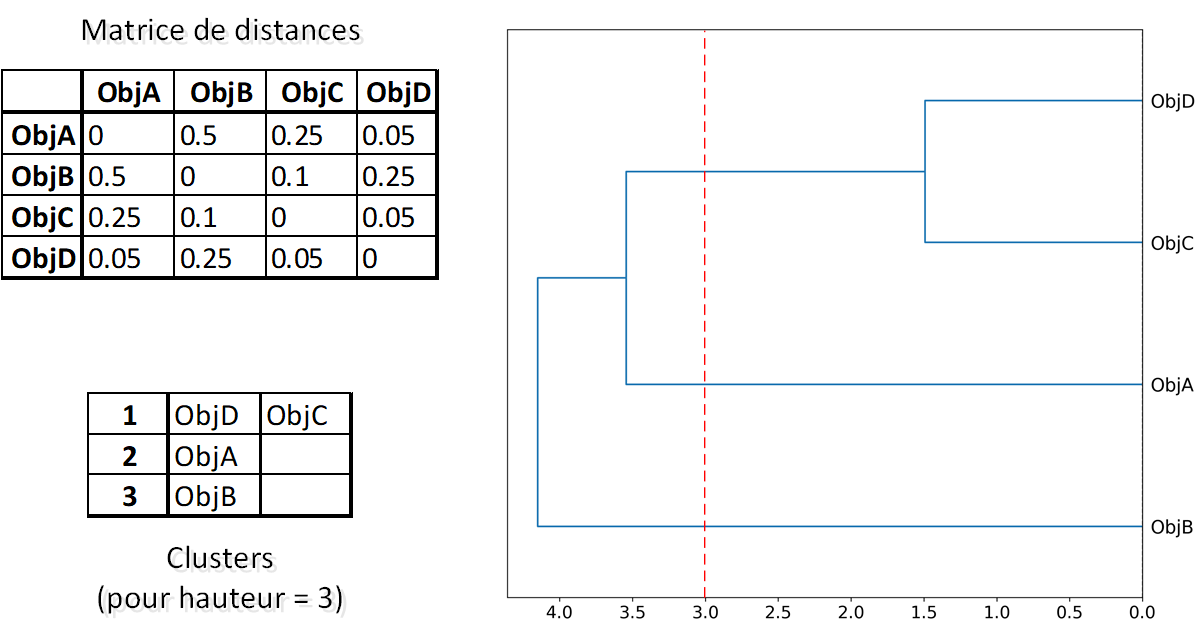
\includegraphics[scale=1]{2-Etat-de-l'Art/images/Clustering/CAH-exemple2.png}
}
\caption{Exemple de construction du dendrogramme et des clusters à la hauteur 3 à partir d'une matrice de distance}
\label{figure:2-S2-Exemple-CAH-Dendrogramme-2}
\end{figure}
%\end{figure*} % Figure flottante
% To use it : fig~\ref{label}





%%%%%%%%%%%%%%%%%%%%%%%%%%%%%%%%%%%%%%%%%%%%%%%%%%%%%%%%%%%%%%%%%%%%%%%%%%%%%%%%%%%%%%%%%%
%%%%%%%%%%%%%%%%%%%%%%%%%%%%%%%%%%%%%%%%%%%%%%%%%%%%%%%%%%%%%%%%%%%%%%%%%%%%%%%%%%%%%%%%%%
%%%%%%%%%%%%%%%%%%%%%%%%%%%%%%%%%%%%%%%%%%%%%%%%%%%%%%%%%%%%%%%%%%%%%%%%%%%%%%%%%%%%%%%%%%
%%%%%%%%%%%%%%%%%%%%%%%%%%%%%%%%%%%%%%%%%%%%%%%%%%%%%%%%%%%%%%%%%%%%%%%%%%%%%%%%%%%%%%%%%%
%%%%%%%%%%%%%%%%%%%%%%%%%%%%%%%%%%%%%%%%%%%%%%%%%%%%%%%%%%%%%%%%%%%%%%%%%%%%%%%%%%%%%%%%%%
%%%%%%%%%%%%%%%%%%%%%%%%%%%%%%%%%%%%%%%%%%%%%%%%%%%%%%%%%%%%%%%%%%%%%%%%%%%%%%%%%%%%%%%%%%

%%%%%%%%%%%%%%%%%%%%%%%%%%%%%%%%%%%%%%%%%%%%
\clearpage % Clean for pictures and tables %
\newpage   % Clean for pictures and tables %
%%%%%%%%%%%%%%%%%%%%%%%%%%%%%%%%%%%%%%%%%%%%

%%%%%%%%%%%%%%%%%%%%%%%%%%%%%%%%%%%%%%%%%%%%%%%%%%%%%%%%%%%%%%%%%%%%%%%%%%%%%%%%%%%%%%%%%%
%%%%%%%%%%%%%%%%%%%%%%%%%%%%%%%%%%%%%%%%%%%%%%%%%%%%%%%%%%%%%%%%%%%%%%%%%%%%%%%%%%%%%%%%%%
%%%%%%%%%%%%%%%%%%%%%%%%%%%%%%%%%%%%%%%%%%%%%%%%%%%%%%%%%%%%%%%%%%%%%%%%%%%%%%%%%%%%%%%%%%
%%%%%%%%%%%%%%%%%%%%%%%%%%%%%%%%%%%%%%%%%%%%%%%%%%%%%%%%%%%%%%%%%%%%%%%%%%%%%%%%%%%%%%%%%%
%%%%%%%%%%%%%%%%%%%%%%%%%%%%%%%%%%%%%%%%%%%%%%%%%%%%%%%%%%%%%%%%%%%%%%%%%%%%%%%%%%%%%%%%%%
%%%%%%%%%%%%%%%%%%%%%%%%%%%%%%%%%%%%%%%%%%%%%%%%%%%%%%%%%%%%%%%%%%%%%%%%%%%%%%%%%%%%%%%%%%


\section{Travaux connexes et similaires}
\label{section:Contexte:TravauxConnexes}

Afin de surmonter les défis rencontrés par les processus à forte intensité de connaissances, et contribuer à la réutilisation de fragments de processus et de leurs connaissances, plusieurs solutions ont été proposées dans la littérature.
Nous présentons maintenant ces solutions et leurs limites, puis nous positionnons notre propre solution.

\bigskip

\subsection{Travaux connexes sur les processus à forte intensité de connaissances}
\label{section:Contexte:TravauxConnexes:KIP}

La réutilisation et les fragments appliqués aux processus à forte intensité de connaissances se retrouvent dans plusieurs travaux.
L'usage de \textit{patterns}, c'est-à-dire des motifs qui se répètent, dans les outils BPM appliqués à des modèles de workflows (BPMN, EPC, ...) est connu et permet de proposer des ensembles de tâches et activités liées et prêtes à l'emploi.

Les travaux présentés dans~\cite{bider2018introducing} visent à expérimenter des patterns dans d'autres types de modèles, en particulier des patterns de buts appliqués au \textit{STate-oriented Business Process Modeling} (SToBPM), où les états sont représentés sous forme d'espace multidimensionnel.
Chaque dimension représente un paramètre, donc un point représente un résultat possible d'une instance de processus.
Si la dimension temporelle est ajoutée, une courbe permet de déterminer l'avancement du processus dans le temps.
Afin de représenter le processus et ses résultats de façon plus adaptée, des formulaires sont préférés en lieu et place de courbes dans des espaces multidimensionnels.
Les buts (et sous-buts) visés par le concepteur, permettant de choisir les patterns dans une bibliothèque, sont construits sur des \textit{décisions} (la finalité à atteindre), des \textit{problèmes} (auxquels appliquer les décisions), des \textit{motivations} (raisons pour lesquelles une décision a été prise, et/ou avancement du problème), des \textit{preneurs de décisions} (organisation, groupe, ou individu), et éventuellement une \textit{date limite} (gestion temporelle).
Un concepteur de processus choisit donc des patterns, s'il le souhaite, en indiquant les buts recherchés dans la bibliothèque.
Il dispose d'une grande liberté pour réutiliser ou non ces patterns, car l'utilisateur n'est pas guidé mais seulement assisté.

Ces travaux illustrent une autre façon de construire des patterns : au lieu de proposer des ensembles d'activités, le concepteur va rechercher des buts à atteindre et les activités nécessaires pour les valider.
La technique de modélisation est cependant beaucoup trop rigide pour être utilisée telle quelle pour des enseignements : bien qu'il soit nécessaire de s'inspirer de sources existantes, le nombre de dimensions finales est inconnu (tous comme le nombre d'états possibles), et les formulaires (ou le découpage en décisions, problèmes, motivations, preneurs de décisions, date limite) ne sont pas du tout adaptés à l'extraction de connaissances.

\bigskip

Dans~\cite{zasada2018box}, on trouve cette fois l'usage de \textit{compliance patterns}~\cite{elgammal2016formalizing} générés à partir de textes légaux pour permettre à des utilisateurs de construire et exécuter des processus respectant les réglementations en place.
La législation sur l'industrie alimentaire a été manuellement analysée afin de sélectionner plusieurs articles, les organiser en catégories et sous-catégories, et y retrouver des patterns fréquents.
Les exigences réglementaires ont ensuite été extraites et transformées en séquences de code, afin de pouvoir les préciser à l'aide des patterns.
Enfin, les patterns ont été formalisés sous forme de formules de \textit{logique linéaire temporelle} (ou \textit{linear temporal logic}/LTL en anglais).

Bien que la méthode puisse être appliquée à d'autres domaines, celle-ci n'est pas encore totalement supportée par les outils informatiques et nécessite plusieurs opérations manuelles.
De plus, il s'agit de patterns construits à partir de textes de loi en langage naturel, donc d'exigences à respecter.
Les supports de cours ayant comme objectif de transmettre des connaissances explicites, ceux-ci n'ont pas vocation à contraindre la conception ou l'exécution d'un processus.
On pourrait tout de même imaginer construire des patterns indiquant dans quel ordre aborder quelles notions lors d'un cours, mais cela implique de s'appuyer sur des textes explicitant ces informations sous forme d'assertions claires et non pas d'un enchaînement de notions comme dans les supports de cours classiques.

\bigskip

Parmi les approches CBR, les travaux présentés dans~\cite{cognini2016case} proposent un langage de modélisation de fragments de processus qui vise à générer et perfectionner manuellement des cas.
Ce langage, nommé \textit{Business Process Feature Model} (BPFM), permet de représenter les cas et leur contenu de façon plus complète que d'autres langages.
Plus spécifiquement, le BPFM est un langage déclaratif capable de représenter des processus partiellement structurés et ordonnés grâce à des contraintes, ainsi que des types de données complexes.
Le point le plus intéressant est sa capacité à représenter des variations de processus.
Les processus sont représentés sous forme d'arbres dont les n\oe{}uds correspondent aux sous-processus, et les feuilles aux activités atomiques.
Les contraintes permettent de déterminer si les activités et sous-processus peuvent ou doivent être utilisés dans les variants du processus, et s'ils peuvent ou doivent être exécutés dans ces variants.
BPFM permet également d'indiquer si des variations apparaissent lors de l'exécution du processus, et de retenir les liens de parentés entre les variations et les modèles initiaux.
Afin de conserver les connaissances liées au processus, l'\textit{Ontology-Based Case-Based Reasoning}~\cite{martin2013integrating} (OBCBR) est utilisée pour conserver les éléments décrivant l'objectif de chaque activité, les rôles de chaque intervenant, et l'auteur de la description du cas.
La réutilisation d'instances passées s'effectue de deux manières : lors de la phase de conception en indiquant les éventuelles variations, lors de l'exécution en modifiant selon les besoins chaque activité ou sous-processus.

Bien que ce langage offre une plus grande liberté d'exécution grâce aux contraintes et aux variations lors de l'exécution, les cas représentés restent fortement orientés du côté des processus métiers structurés : on représente un processus par un arbre de sous-processus et d'activités qui s'enchaînent.
Dans le cadre de la construction d'un cours, le syllabus pourrait être représenté sous forme d'arbre où les chapitres et sections formeraient différents niveaux, cependant, les connaissances que l'on cherche à transmettre ne sont pas de simples activités qu'il suffit de mentionner pour pouvoir les valider.
La réutilisation de cours passés implique d'assister à chaque cours ou de lire intégralement le contenu pour le modéliser, puis l'intégrer au modèle BPFM.
La difficulté réside dans l'association de certaines notions les unes avec les autres : il n'est pas possible en l'état de découvrir facilement les contraintes dans l'ordre des notions entre chaque variation de cours, car il s'agit de connaissances implicites à chaque enseignant.

\bigskip

Afin de mieux renseigner les gabarits réutilisables, les travaux dans~\cite{tenschert2016supporting} explorent l'usage de l'\textit{Acte de Langage} (ou \textit{Speech Act Theory} en anglais).
L'excès de gabarits, et le manque d'informations ou leur trop courte description pour les discerner clairement les uns des autres, implique que l'utilisateur doit rechercher lui-même l'objectif de chaque gabarit pour sélectionner le plus adapté à son cas.
Afin de retrouver plus rapidement le gabarit le plus adapté, les interactions et micro-processus sont analysés.
Un micro-processus est composé d'actes de coordination (équivalent de méta-données décrivant ce que le micro-processus vise à faire, qui l'exécute, envers quelle(s) autre(s) personne(s), le support, l'horodatage, le contenu, et d'autres annotations) et d'actes de production (création d'un artefact).
Les micro-processus s'appuient sur les actes de langage pour décrire toutes les informations des actes de coordination.
L'intérêt des micro-processus repose sur la possibilité laissée aux utilisateurs du métier de créer leurs propres gabarits selon les interactions qu'ils utilisent le plus souvent sans être perdus parmi d'immenses bibliothèques de gabarits.
Les connaissances tacites sont ainsi plus facilement mises à contribution dans les nombreuses méta-données des actes de coordination : les utilisateurs du métier emploient leur vocabulaire et modélisent leurs activités depuis leur propre point de vue, ils sont ainsi plus facilement capables de retrouver et réutiliser leurs propres gabarits.

Bien que ces travaux n'embarquent pour le moment qu'un petit sous-ensemble d'objets par rapport à ce que la gestion de cas préconise (documents, contacts, communications, ...), laisser les utilisateurs créer eux-mêmes des gabarits réutilisables à partir de leurs propres connaissances simplifie l'usage de la solution présentée.
Une limitation soulevée en conclusion dans~\cite{tenschert2016towards} indique que cette solution ne peut fonctionner que si les utilisateurs acceptent de renseigner chacun des micro-processus qu'ils utilisent.
Dans le cas de la construction de cours, on retrouve une limitation très proche : pour pouvoir réutiliser les supports de cours d'autres enseignants, il faut que tous les enseignants utilisent le même outil pour y insérer leurs connaissances.
Bien que PowerPoint et ses équivalents libres soient très fréquents, ceux-ci sont très rarement utilisés avec l'ensemble des fonctionnalités qui se rapprochent de la contribution décrite dans~\cite{tenschert2016supporting} (par exemple, les schémas sont souvent de simples images importées, et les méta-données des objets PowerPoint ne sont quasiment jamais renseignées).
Cependant, le vocabulaire du domaine et certaines activités (tels que les travaux dirigés ou pratiques) sont présents dans les diapositives qui peuvent être réutilisées à postériori par d'autres enseignants.

\bigskip

Du point de vue de la gestion des connaissances appliquée à la gestion de projets, une solution sur la réutilisation des connaissances est proposée dans~\cite{schacht2016methodology}.
Celle-ci se compose de trois parties :

\begin{itemize}
\item Un double-cycle dont la boucle choisie dépend du contexte de l'organisation et de l'équipe.
Récapitulatif : à la fin de chaque projet, l'équipe se réunit pour transférer son expérience aux autres équipes.
Préparation : au démarrage du projet ou d'une étape importante (c'est-à-dire \textit{pendant} le projet), l'équipe se réunit pour réfléchir à la conception de la solution à partir de l'expérience de chaque membre.

\item De nouveaux rôles sont définis pour retenir et transférer les expériences des équipes.
L'expert en leçons (\textit{lessons learned expert} en anglais) qui dispose de compétences pour traiter les connaissances et expériences issues de la réalisation du projet.
L'expert du sujet (\textit{topic expert} en anglais) qui dispose de connaissances et d'expérience sur le sujet traité par le projet.

\item Un processus centré sur les connaissances appliqué à la gestion de projet (\textit{knowledge-centric project management process} en anglais) s'appuyant sur le PMBOK\copyright ~du \textit{Project Management Institute}.
\end{itemize}

Dans le contexte récapitulatif, l'équipe doit se souvenir des évènements clés qui ont eu un impact sur le résultat du projet (succès ou échec).
Chaque évènement est ensuite analysé pour en déterminer les causes et les retenir.
L'ensemble de ces connaissances est enregistré dans un dépôt partagé, puis un membre de l'équipe est chargé de surveiller l'apparition de ces évènements lors des projets suivants.
À l'inverse, dans le contexte de préparation, les risques sont évalués en amont grâce à l'expérience de chaque membre (ou des sources de connaissances les plus adaptées au projet) et peuvent être pris en charge par les techniques de gestion des risques.
Le processus général proposé s'appuie en pratique sur plusieurs itérations de la double boucle.
Lors du démarrage du projet, la boucle de \textit{préparation} est effectuée une première fois.
À chaque étape clé, un cycle \textit{récapitulatif} et un cycle de \textit{préparation} sont effectués pour tirer les leçons nécessaires de l'étape terminée et continuer à progresser vers l'étape suivante.
Enfin, lorsque le projet se termine, un cycle \textit{récapitulatif} est effectué pour conserver toutes les connaissances.
Les deux rôles d'experts interviennent soit pour gérer le processus dans son ensemble (expert en leçons), soit pour traiter les connaissances liées à l'étape en cours (expert du sujet).

Cette solution et son processus permettant d'apprendre des expériences passées sont intéressants, mais il faut néanmoins l'adapter au domaine visé.
Dans le cadre de l'enseignement et des cours, on retrouve ce processus sous une forme plus simplifiée : l'enseignant construit tout d'abord son cours en amont (éventuellement en s'appuyant sur l'expérience des précédents semestres où il l'a enseigné), à la fin de chaque séance il note les difficultés rencontrées avec les groupes, puis adapte ses séances suivantes.
Un autre point de vue de plus haut niveau est aussi accessible : une phase exclusivement préparatoire s'appuyant sur les expériences passées (les siennes ou celles de ses collègues) sera exécutée, puis, à chaque semestre où il enseignera de nouveau son cours, il pourra effectuer un récapitulatif du semestre précédent et préparer le suivant.


\bigskip

%%%%%%%%%%%%%%%%%%%%%%%%%%%%%%%%%%%%%%%%%%%%
%\clearpage % Clean for pictures and tables %
%\newpage   % Clean for pictures and tables %
%%%%%%%%%%%%%%%%%%%%%%%%%%%%%%%%%%%%%%%%%%%%


\subsection{Positionnement de la méthode CREA}
\label{section:Contexte:TravauxConnexes:PositionnementCREA}

Comme nous venons de le voir, plusieurs solutions sur la réutilisation de fragments de processus (contenant des connaissances tacites) ont été proposées dans la littérature mais ne peuvent pas directement être utilisées dans le cas de la construction d'un cours dans l'enseignement supérieur.
Le processus proposé dans~\cite{schacht2016methodology} se divise en deux étapes : préparation puis récapitulatif.
La préparation implique de s'inspirer des expériences passées pour prévoir les difficultés rencontrées.
On retrouve partiellement cette vision dans le raisonnement à base de cas où un (ou des) cas passé(s) ser(ven)t de base pour le cas courant.
Il s'agit donc de s'appuyer sur les expériences passées, et leurs productions, pour répondre au problème actuel.
La méthode CREA, \textit{\MyCREA}, que nous proposons s'intéresse particulièrement à l'extraction et l'analyse de connaissances à partir de documents issus d'instances passées pour proposer des scénarios de réutilisation possibles.

\bigskip

Les supports de cours produits par les enseignants sont assimilables à une explicitation des connaissances où subsiste malgré tout une certaine expertise tacite : le choix précis des notions et de leur enchaînement est directement lié à l'enseignant et sa propre expérience qu'il compte mettre à profit des étudiants.
Les documents ainsi produits par les enseignants peuvent donc être traités comme des artefacts de cas passés.
Ces documents étant rédigés en langage naturel, pour pouvoir en extraire des informations et connaissances réutilisables, il est nécessaire d'employer tout d'abord des techniques de TAL.
BabelFy et BabelNet permettant de s'appuyer sur des bases de connaissances très populaires et communes à l'humanité, leur usage répond parfaitement aux besoins de la gestion des connaissances concernant l'usage d'un vocabulaire commun.
Le point de vue des cas employé par ACM et CBR implique d'analyser et réutiliser les connaissances des cas, pour cela, nous employons l'ACF qui permet de découvrir des connaissances tacites parmi les documents et les textes les composant (en particulier les liens entre eux).
Ce couple base de connaissances partagée et ACF pour analyser des documents ayant déjà été approuvés par des travaux de thèse~\cite{tang2016interactive}, leur usage à des fins de réutilisation du contenu de ces documents est donc tout à fait approprié.

Bien qu'il soit impossible de manipuler directement les connaissances tacites, il est néanmoins possible de les manipuler indirectement grâce aux métriques présentées dans une autre thèse~\cite{jaffal2019aide}, en particulier avec l'impact mutuel et la similarité conceptuelle.
Une fois l'extraction et l'analyse réalisées, il est nécessaire de ré-assembler les informations et connaissances pour qu'un enseignant (l'expert) puisse les adapter à son cours (son cas), pour cela, nous employons des techniques de clustering sur la similarité conceptuelle des termes dans les documents.
L'enseignant se voit proposer des groupes de notions pertinents issus de précédents cours.
Afin que la pertinence soit maximale, il est nécessaire que l'enseignant insère lui-même uniquement des supports de cours traitant du même sujet.
Cependant, si quelques documents traitent de sujets trop éloignés, l'impact mutuel sera capable d'identifier ces documents et indiquer à l'enseignant lesquels devraient être retirés.

\bigskip

La méthode CREA s'insère donc parfaitement dans la partie réutilisation de la gestion des connaissances et de la gestion de cas (ACM et CBR en particulier dans cette thèse) : des connaissances sont retrouvées, préparées, sélectionnées, et réutilisées.
L'enseignant est ensuite libre d'adapter les clusters proposés à son propre cas.
Il peut néanmoins supprimer des notions qui ne l'intéressent pas, et relancer une partie de la méthode pour obtenir de nouveaux résultats plus proches de ses attentes.
